\documentclass[aspectratio=169,11pt,xcolor=table]{beamer}

% =========================================================
% PACKAGES
% =========================================================
\usepackage[utf8]{inputenc}
\usepackage[T1]{fontenc}
\usepackage{lmodern}
\usepackage{amsmath,amssymb}
\usepackage{booktabs}
\usepackage{array}
\usepackage{tikz}
\usepackage{ragged2e}
\usepackage{graphicx}
\usepackage{animate}
\usepackage[table]{xcolor}
\usepackage{hyperref}
\usepackage{booktabs}
\usepackage{array}
\usepackage[table]{xcolor}
\usetikzlibrary{
    arrows.meta,
    positioning,
    shapes.geometric,
    shapes.misc,
    fit,
    calc
}

% =========================================================
% COLORS
% =========================================================

\definecolor{AmritaMaroon}{RGB}{165,0,55}
\definecolor{AmritaDark}{RGB}{95,0,35}
\definecolor{LightBlue}{RGB}{220,237,250}
\definecolor{LightGreen}{RGB}{224,244,228}
\definecolor{LightOrange}{RGB}{252,235,205}
\definecolor{LightPink}{RGB}{250,225,235}
\definecolor{LightGray}{RGB}{242,242,242}

% Add these missing color definitions:
\definecolor{LightCyan}{RGB}{224,255,255}
\definecolor{LightYellow}{RGB}{255,255,224}
% THEME
% =========================================================
\usetheme{default}

\setbeamertemplate{navigation symbols}{}

\setbeamertemplate{frametitle}{
    \vspace{0.15cm}
    \begin{beamercolorbox}[
        wd=\paperwidth,
        ht=0.85cm,
        dp=0.15cm,
        leftskip=0.35cm
    ]{frametitle}
        \color{white}
        \Large\insertframetitle
    \end{beamercolorbox}
}

\setbeamercolor{frametitle}{bg=AmritaMaroon}
\setbeamercolor{normal text}{fg=black}
\setbeamercolor{structure}{fg=AmritaMaroon}

% =========================================================
% CUSTOM COMMANDS
% =========================================================

\newcommand{\subtitleline}[1]{
    \vspace{-0.05cm}
    {\small\color{AmritaDark}\textit{#1}}
    \vspace{0.15cm}
}

\newcommand{\highlight}[1]{
    \textbf{\color{AmritaMaroon}#1}
}

\newcommand{\bulletitem}[2]{
    \item \textbf{#1} #2
}

\newcommand{\infobox}[4]{
    \begin{tikzpicture}
        \node[
            rounded corners=5pt,
            fill=#1,
            inner sep=9pt,
            text width=#2
        ] {
            \textbf{\color{AmritaMaroon}#3}\\[3pt]
            #4
        };
    \end{tikzpicture}
}


\newcommand{\ROoneSent}{Privacy-preserving single-modality sensing to separate daily Activities from Sign Gestures.}
\newcommand{\ROtwoSent}{Single-person, multi-modality recognition of complex interleaved activities.}
\newcommand{\ROthreeSent}{Multi-person, multi-modality recognition of parallel and concurrent activities.}
\newcommand{\ROfourSent}{Multimodal fusion for context- and intent-aware smart-home control.}

\setbeamercolor{robox}{bg=LightGray,fg=AmritaMaroon}

% Compact RO banner: kept close to one \small line in height so that
% dense slides retain their original vertical budget.
\newcommand{\robox}[1]{%
    \vspace{-0.12cm}%
    \begin{beamercolorbox}[
        wd=0.965\textwidth,
        sep=4pt,
        rounded=true
    ]{robox}
        \scriptsize #1
    \end{beamercolorbox}%
    \vspace{0.10cm}%
}

\newcommand{\roone}{\robox{\textbf{RO1:} \ROoneSent}}
\newcommand{\rotwo}{\robox{\textbf{RO2:} \ROtwoSent}}
\newcommand{\rothree}{\robox{\textbf{RO3:} \ROthreeSent}}
\newcommand{\rofour}{\robox{\textbf{RO4:} \ROfourSent}}
\newcommand{\roonefour}{\robox{\textbf{RO1:} \ROoneSent\\[2pt] \textbf{RO4:} \ROfourSent}}

\newcommand{\rotag}[1]{
    \begin{tikzpicture}[remember picture,overlay]
        \node[
            anchor=north east,
            fill=white,
            text=AmritaMaroon,
            rounded corners=2pt,
            inner xsep=4pt,
            inner ysep=2pt,
            font=\scriptsize\bfseries
        ] at ([xshift=-0.35cm,yshift=-0.28cm]current page.north east) {#1};
    \end{tikzpicture}%
}

% =========================================================
% TITLE
% =========================================================

\title{
    \textbf{Multimodal Human Activity}\\
    \textbf{and Sign Language Recognition for Inclusive Smart Homes}
}

\author{
    23CSE399 -- Project Phase 2\\[3mm]
    \small
    Adhikkesh S K \quad
    Adithya Ajay \quad
    Amrith B\\
    Gowreesh B \quad
    Rishiikesh S K
}

\institute{
    Department of Computer Science and Engineering\\
    Amrita Vishwa Vidyapeetham
}

\date{
    Guide Review 1 \;|\; Panel Review 1
}

% =========================================================
% DOCUMENT
% ====


% Self-contained PDF animations; each page of the frame PDF is one frame.
% The supplied media are preconverted, so Overleaf needs no shell escape.
\newcommand{\implclip}[2]{%
  \animategraphics[type=pdf,method=widget,autoplay,loop,autopause,
    controls={play,stop},buttonsize=0.17cm,
    width=\linewidth,height=#2,keepaspectratio,poster=first,label=#1]
    {8.333333}{current_impl/media/#1_frames}{}{}%
}
\newcommand{\implnote}[1]{{\scriptsize\color{AmritaDark}#1\par}}

\begin{document}


% =========================================================
% TITLE SLIDE
% =========================================================

\begin{frame}
    \begin{tikzpicture}[remember picture,overlay]

        % Top label
        \node[
            anchor=north east,
            fill=AmritaMaroon,
            text=white,
            rounded corners=3pt,
            inner xsep=10pt,
            inner ysep=5pt
        ] at ([xshift=-0.25cm,yshift=-0.2cm]current page.north east)
        {\scriptsize Type 2: Application Project};

    \end{tikzpicture}

    \vspace{0.7cm}

    \begin{center}
        {\color{AmritaMaroon}\Large\bfseries
        Multimodal Human Activity and}\\[0.15cm]    

        {\color{AmritaMaroon}\LARGE\bfseries
        Sign Language Recognition for Inclusive Smart Homes}

        \vspace{0.45cm}

        {\large 23CSE399 -- Project Phase 2}\\
        {\large Guide Review 1 \;|\; Panel Review 1}

        \vspace{0.45cm}

        \begin{tabular}{c}
        Adhikkesh S K\\
        Adithya Ajay\\
        Amrith B\\
        Gowreesh B\\
        Rishiikesh S K
        \end{tabular}

        \vspace{0.35cm}

        \textbf{Guide: Ms. Nalinadevi K}\\
        Department of CSE, Amrita Vishwa Vidyapeetham
    \end{center}
\end{frame}

\begin{frame}{ Guide Approval}

\begin{center}

\vspace{0.15cm}

\includegraphics[
    width=0.82\textwidth,
    height=0.70\textheight,
    keepaspectratio
]{Approval.png}

\vspace{0.12cm}

{\small\color{AmritaDark}
\textit{Guide approval}
}

\end{center}

\end{frame}

% =========================================================
% 1. USE CASES
% =========================================================

\begin{frame}{1. Motivation}

\begin{itemize}
    \setlength{\itemsep}{0.45em}
    \setlength{\parskip}{0pt}

    \item \textcolor{blue}{\textbf{Smart Homes:}}
    Rapid adoption --- \textbf{82.1\% projected increase in smarthome systems by 2026}
    \hspace{0.2em}\textit{\small (Statista)}

    \item \textcolor{blue}{\textbf{Accessibility:}}
    \textbf{1.5 billion} people with hearing loss
    $\rightarrow$ \textbf{2.5 billion by 2050}
    \hspace{0.1em}\textit{\small (WHO)}

    \item \textcolor{blue}{\textbf{Sign-Language Recognition:}}
    Since \textbf{1991} --- predominantly
    \textbf{camera/image- or wearable sensor-based recognition}

    \item \textcolor{blue}{\textbf{Human Activity Recognition:}}
    Predominantly \textbf{single-modality sensing}
    $\rightarrow$ limited information from one sensing source

    \item \textcolor{blue}{\textbf{Privacy:}}
    \textbf{87\% of reviewed studies} reported privacy concerns
    with smart-home surveillance
    \hspace{0.2em}\textit{\small (JMIR Scoping Review)}

\end{itemize}

\vspace{0.2cm}

\begin{beamercolorbox}[
    rounded=true,
    sep=0.6em,
    wd=\textwidth
]{block body}

\small
Most existing systems rely on \textbf{single-modality sensing},
limiting recognition of \textbf{activities, sign language, interactions,
and intent}. Along with \textbf{camera privacy concerns} and the need
for \textbf{accessible smart homes}, this motivates a
\textbf{multimodal, privacy-preserving approach}.

\end{beamercolorbox}

\end{frame}


% =========================================================
% 2. USE CASE 3
% =========================================================

\begin{frame}{2. Introduction}

\begin{itemize}
    \setlength{\itemsep}{0.5em}

    \item \textcolor{blue}{\textbf{Context Awareness:}}
    \textit{What is happening?}
    $\rightarrow$ Person sitting, walking, cooking

    \item \textcolor{blue}{\textbf{Intent Awareness:}}
    \textit{Why is it happening?}
     Opening a door → To leave, to let a guest in, to get fresh air

    \item \textcolor{blue}{\textbf{Context $\neq$ Intent:}}
    The same activity can represent \textbf{different intentions}
    depending on the situation.

    \item \textcolor{blue}{\textbf{Real-World Complexity:}}
    \textbf{Multiple people + simultaneous activities + interactions}
    make intent harder to infer.

    \item \textcolor{blue}{\textbf{Beyond Activity Recognition:}}
    Understanding \textbf{who is doing what, with whom, and why}
    enables more meaningful automation.

    \item \textcolor{blue}{\textbf{Our Goal:}}
    Move from \textbf{activity recognition}
    $\rightarrow$ \textbf{context understanding}
    $\rightarrow$ \textbf{intent-aware smart-home decisions}.
\end{itemize}

\end{frame}
% =========================================================
% 4. LITERATURE SURVEY: HUMAN ACTIVITY RECOGNITION (HAR)
% =========================================================

\begin{frame}[t]{3. Literature Survey: Human Activity Recognition (HAR)}

\vspace{-0.1cm} % Lift to maximize space
\centering
\fontsize{5.5}{6.5}\selectfont
\renewcommand{\arraystretch}{1.05} % Healthier row spacing
\setlength{\tabcolsep}{3pt}

\begin{tabular}{
>{\bfseries\RaggedRight\arraybackslash}m{0.12\textwidth}
>{\RaggedRight\arraybackslash}m{0.20\textwidth}
>{\RaggedRight\arraybackslash}m{0.10\textwidth}
>{\RaggedRight\arraybackslash}m{0.22\textwidth}
>{\RaggedRight\arraybackslash}m{0.30\textwidth} % Widened to reduce line breaks
}

\rowcolor{AmritaMaroon}
{\color{white}\textbf{Paper / Year / Author}} &
{\color{white}\textbf{Problem Addressed}} &
{\color{white}\textbf{Dataset}} &
{\color{white}\textbf{Technique}} &
{\color{white}\textbf{Result \& Limitation}} \\

\arrayrulecolor{white}\hline

\rowcolor{LightBlue}
\textbf{LAHAR}\newline \textnormal{(2024)}\newline \textnormal{Chen et al.~[1]} &
Differentiating multiple people and recognizing concurrent activities. &
Ambient\newline\textit{(Sensor Logs)} &
Converts sensor events into text and uses an LLM to reason about activities. &
\textbf{Result:} Strong performance on ARAS multi-person data.\newline
\textbf{Limit:} Lacks fine hand/finger motion detection, creating context blindness. \\

\hline

\rowcolor{LightGreen}
\textbf{Multi-Skel}\newline \textnormal{(2024)}\newline \textnormal{Li et al.~[2]} &
Reducing the complexity of multi-person tracking while preserving accuracy. &
Video / Skel\newline\textit{(Vision)} &
Detects and tracks skeleton keypoints for several people from video. &
\textbf{Result:} 98.0\% accuracy with improved tracking on MOT16.\newline
\textbf{Limit:} Body occlusion hides keypoints, reducing reliable recognition. \\

\hline

\rowcolor{LightCyan}
\textbf{PA-CSI}\newline \textnormal{(2025)}\newline \textnormal{Quy et al.~[3]} &
Combining WiFi amplitude and phase for robust activity recognition. &
WiFi CSI\newline\textit{(RF Signals)} &
Combines WiFi amplitude and phase through attention-based fusion. &
\textbf{Result:} 99.9\% in-room and 98.0\% unseen room accuracy.\newline
\textbf{Limit:} High accuracy, but motion from multiple people overlaps in RF signals. \\

\hline

\rowcolor{LightOrange}
\textbf{Interact-Obj}\newline \textnormal{(2025)}\newline \textnormal{Wen et al.~[4]} &
Using interacted objects to improve recognition beyond skeletal features. &
RGB-D\newline\textit{(Skel+Obj)} &
Adds the interacted object as an extra node in the skeleton graph. &
\textbf{Result:} 96.7\% cross-subject and 99.2\% cross-view on NTU-60.\newline
\textbf{Limit:} Vision-based system still struggles with simultaneous actions. \\

\hline

\rowcolor{LightPink}
\textbf{AttCLHAR}\newline \textnormal{(2024)}\newline \textnormal{Ref.~[5]} &
Suppressing noisy skeletal features to improve activity recognition. &
Wearable\newline\textit{(IMU Sensors)} &
Uses self-attention over wearable accelerometer and gyroscope signals. &
\textbf{Result:} 98.1\% on WISDM and 96.0\% on USC-HAD.\newline
\textbf{Limit:} Wearable signals provide little context about surrounding people. \\

\hline

\rowcolor{LightYellow}
\textbf{OAHR}\newline \textnormal{(2024)}\newline \textnormal{Ref.~[6]} &
Maintaining recognition when some skeleton joints are hidden or missing. &
Skeleton\newline\textit{(Occluded)} &
Represents the skeleton as a 3D volume to handle missing joints. &
\textbf{Result:} 97.1\% on NTU RGB+D 60 with occlusion robustness.\newline
\textbf{Limit:} Vision-based; does not provide privacy-safe multi-user separation. \\

\end{tabular}

\vspace{0.15cm}

\setlength{\fboxrule}{0.75pt}
\setlength{\fboxsep}{4pt}
\fcolorbox{AmritaMaroon}{white}{%
\begin{minipage}{0.94\textwidth}
{\color{AmritaMaroon}\fontsize{5.5}{6.5}\selectfont\textbf{Research Gap: }}
{\fontsize{5.5}{6.5}\selectfont
Single-modality systems suffer from context blindness, while vision-based frameworks can degrade under occlusion or multi-user overlap. The use of LLMs, object-aware skeletons, and attention-based learning shows progress, but a \textbf{robust multimodal fusion framework} is still needed for complex parallel activities.
}
\end{minipage}%
}

\end{frame}

% =========================================================
% 5. LITERATURE SURVEY: SIGN LANGUAGE RECOGNITION
% =========================================================

\begin{frame}[t]{4. Literature Survey: Sign Language Recognition}

\vspace{-0.1cm} % Lift to maximize space
\centering
\fontsize{5.5}{6.5}\selectfont
\renewcommand{\arraystretch}{1.05} % Healthier row spacing
\setlength{\tabcolsep}{3pt}

\begin{tabular}{
>{\bfseries\RaggedRight\arraybackslash}m{0.12\textwidth}
>{\RaggedRight\arraybackslash}m{0.20\textwidth}
>{\RaggedRight\arraybackslash}m{0.10\textwidth}
>{\RaggedRight\arraybackslash}m{0.22\textwidth}
>{\RaggedRight\arraybackslash}m{0.30\textwidth} % Widened to reduce line breaks
}

\rowcolor{AmritaMaroon}
{\color{white}\textbf{Paper / Year / Author}} &
{\color{white}\textbf{Problem Addressed}} &
{\color{white}\textbf{Dataset}} &
{\color{white}\textbf{Technique}} &
{\color{white}\textbf{Result \& Limitation}} \\

\arrayrulecolor{white}\hline

\rowcolor{LightBlue}
\textbf{SignFi}\newline \textnormal{(2018)}\newline \textnormal{Ma et al.~[7]} &
Camera-free sign gesture recognition in home settings. &
SignFi\newline\textit{(WiFi CSI)} &
CNN tracking hand/finger motion from WiFi signal variations. &
\textbf{Result:} 98.9\% (known), 86.6\% (unseen).\newline
\textbf{Limit:} Nearby motion corrupts target sign signal. \\

\hline

\rowcolor{LightGreen}
\textbf{CorrNet}\newline \textnormal{(2023)}\newline \textnormal{Hu et al.~[8]} &
Tracking hand and face movements in continuous video. &
PHOENIX\newline\textit{(RGB Video)} &
Correlates hand and face regions without explicit pose estimation. &
\textbf{Result:} 19.4\% Word Error Rate.\newline
\textbf{Limit:} Vulnerable to occlusion and privacy issues. \\

\hline

\rowcolor{LightCyan}
\textbf{LLMs SLT}\newline \textnormal{(2024)}\newline \textnormal{Gong et al.~[9]} &
Connecting visual sign tokens to LLMs for translation. &
PHOENIX\newline\textit{(RGB Video)} &
Converts sign video into discrete tokens for LLM translation. &
\textbf{Result:} BLEU-1 45.2 vs 33.2 baseline.\newline
\textbf{Limit:} Camera-based; fails with background motion. \\

\hline

\rowcolor{LightOrange}
\textbf{Wi-SL}\newline \textnormal{(2023)}\newline \textnormal{Wang et al.~[10]} &
Extracting fine hand motion from noisy WiFi CSI. &
Custom\newline\textit{(WiFi CSI)} &
CNN processing with nearest-neighbor matching across rooms. &
\textbf{Result:} 98.9\% gesture accuracy.\newline
\textbf{Limit:} Single-signer focus; overlapping degrades performance. \\

\hline

\rowcolor{LightPink}
\textbf{WatchSign}\newline \textnormal{(2023)}\newline \textnormal{Liu et al.~[11]} &
Daily sign language recognition using wearable devices. &
Custom\newline\textit{(Wearable IMU)} &
Smartwatch and smart ring sensors capture wrist/finger motion. &
\textbf{Result:} 94.2\% accuracy on 100 ASL words.\newline
\textbf{Limit:} Cannot detect ambient multi-person activities. \\

\hline

\rowcolor{LightYellow}
\textbf{ASL Trans.}\newline \textnormal{(2024)}\newline \textnormal{Gu et al.~[12]} &
Continuous sentence-level ASL translation without cameras. &
Custom\newline\textit{(Wearable IMU)} &
Wearable inertial motion capture decoded via Bi-LSTM. &
\textbf{Result:} 99.0\% word, 97.3\% sentence accuracy.\newline
\textbf{Limit:} Full-body suit is too intrusive for daily home use. \\

\hline

\rowcolor{LightCyan}
\textbf{RF-ASLR}\newline \textnormal{(2026)}\newline \textnormal{Nosheen et al.~[13]} &
Privacy-preserving sign language recognition via RF sensing. &
Custom\newline\textit{(Wireless CSI)} &
Software-defined radio CSI temporal patterns decoded via LSTM. &
\textbf{Result:} 98.0\% accuracy across 20 ASL signs.\newline
\textbf{Limit:} Tested only in controlled, static, single-user setups. \\

\end{tabular}

\vspace{0.15cm}

\setlength{\fboxrule}{0.75pt}
\setlength{\fboxsep}{4pt}
\fcolorbox{AmritaMaroon}{white}{%
\begin{minipage}{0.94\textwidth}
{\color{AmritaMaroon}\fontsize{5.5}{6.5}\selectfont\textbf{Research Gap: }}
{\fontsize{5.5}{6.5}\selectfont
Existing single-modality models (WiFi CSI, Vision, IMU) suffer performance drops amid multi-person background activity. A \textbf{multimodal fusion framework} combining WiFi CSI with complementary contactless sensing is required to isolate sign language intent from environmental interference while maintaining privacy.
}
\end{minipage}%
}

\end{frame}
% =========================================================
% 6. Problem Statement
% ========================================================
\begin{frame}{5. Problem Statement}

\vspace{0.1cm}
\centering

% --- Box 1: Challenge ---
\begin{tikzpicture}
\node[
    rounded corners=10pt,
    fill=structure.fg!4,
    draw=structure.fg!45,
    line width=0.7pt,
    minimum width=0.92\textwidth,
    inner sep=14pt,
    text width=0.82\textwidth,
    align=justify
] {
    \small
    \textbf{Challenge:}\\[0.15cm]
    How can smart homes reliably recognize intentional
    communicative gestures without relying on intrusive
    camera-based sensing?
};
\end{tikzpicture}

\vspace{0.3cm} % Space between the two boxes

% --- Box 2: Problem Statement ---
\begin{tikzpicture}
\node[
    rounded corners=10pt,
    fill=structure.fg!4,
    draw=structure.fg!45,
    line width=0.7pt,
    minimum width=0.92\textwidth,
    inner sep=14pt,
    text width=0.82\textwidth,
    align=justify
] {
    \small
    \textbf{Problem Statement:}\\[0.15cm]
    To build a privacy-preserving multimodal sensing system that distinguishes routine activities from intentional non-verbal communication, understands user intent through contextual information, and enables appropriate smart-home control without relying on intrusive camera-based sensing.
};
\end{tikzpicture}

\end{frame}
% ========================================================


% =========================================================
% 6. RESEARCH OBJECTIVES
% =========================================================

\begin{frame}{6. Research Objectives}
\justifying
\small
\begin{itemize}
    \item \textbf{RO1:} To design a privacy-preserving, single-person, single-modality data acquisition methodology, and to develop classification models that distinguish daily \textit{Activities} from \textit{Sign Gestures}.

    \item \textbf{RO2:} To extend this methodology to a single-person, multi-modality setting, and develop classification models that accurately recognize complex, interleaved activities performed by a single individual.

    \item \textbf{RO3:} Extension to multi-person, multi-modality sign and activity recognition system  capable of accurately identifying  parallel and concurrent activities across multiple individuals within a shared environment.

    \item \textbf{RO4:} To develop multimodal fusion strategies that establish comprehensive context and intent awareness, seamlessly translating deliberate non-verbal communication into privacy-preserving smart home controls.
\end{itemize}
\end{frame}

% =========================================================
% 7. PROJECT TIMELINE (ROAD-STYLE)
% =========================================================

\begin{frame}{7. Project Timeline: Progress \& 3-Month Roadmap}

\vspace{-0.05cm}

\begin{center}

\begin{tikzpicture}
\node[
    fill=AmritaMaroon,
    minimum width=0.42\textwidth,
    minimum height=0.6cm,
    align=center,
    text=white,
    font=\bfseries\small,
    rounded corners=4pt
] (bar60) {60\% COMPLETE};

\node[
    fill=LightOrange,
    draw=AmritaMaroon,
    thick,
    minimum width=0.42\textwidth,
    minimum height=0.6cm,
    align=center,
    text=AmritaMaroon,
    font=\bfseries\small,
    rounded corners=4pt,
    right=1pt of bar60
] (bar40) {NEXT 3 MONTHS --- 40\% PENDING};
\end{tikzpicture}
\end{center}

\vspace{0.15cm}

\resizebox{0.98\textwidth}{!}{%
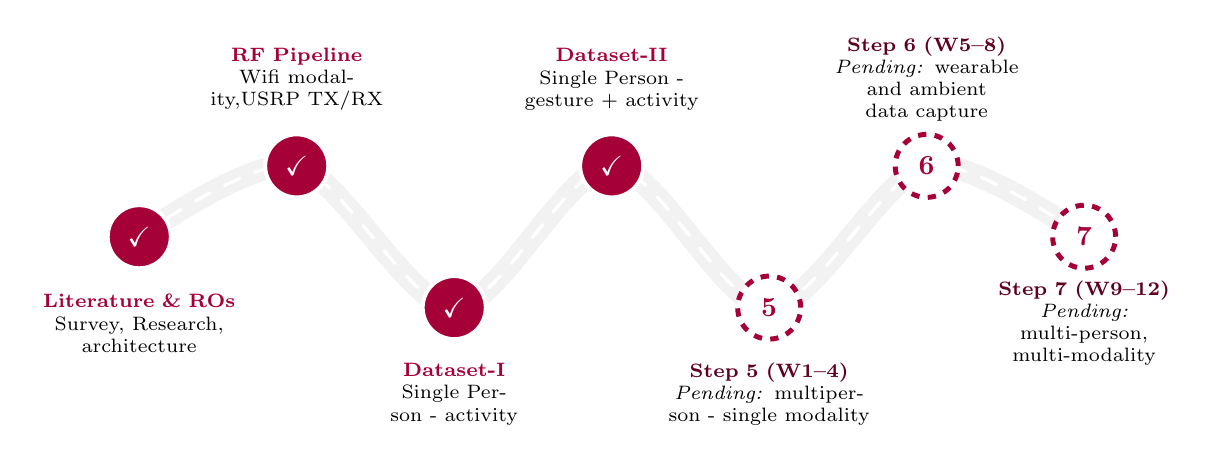
\begin{tikzpicture}

% ---------- ROAD PATH COORDINATES ----------
\coordinate (P1) at (0,0);
\coordinate (P2) at (2.0,0.9);
\coordinate (P3) at (4.0,-0.9);
\coordinate (P4) at (6.0,0.9);
\coordinate (P5) at (8.0,-0.9);
\coordinate (P6) at (10.0,0.9);
\coordinate (P7) at (12.0,0);

% ---------- ROAD SURFACE ----------
\draw[line width=8pt, LightGray, line cap=round]
    plot[smooth] coordinates {(P1) (P2) (P3) (P4) (P5) (P6) (P7)};
\draw[line width=1.2pt, white, dash pattern=on 6pt off 6pt, line cap=round]
    plot[smooth] coordinates {(P1) (P2) (P3) (P4) (P5) (P6) (P7)};

% ---------- NODE STYLES ----------
\tikzset{
  donecirc/.style={
    circle, fill=AmritaMaroon, draw=white, line width=1.4pt,
    minimum size=0.8cm, font=\bfseries\color{white}
  },
  pendcirc/.style={
    circle, fill=white, draw=AmritaMaroon, line width=1.8pt, dashed,
    minimum size=0.8cm, font=\bfseries\color{AmritaMaroon}
  }
}

% ---------- STEP MARKERS ----------
\node[donecirc] at (P1) {\checkmark};
\node[donecirc] at (P2) {\checkmark};
\node[donecirc] at (P3) {\checkmark};
\node[donecirc] at (P4) {\checkmark};
\node[pendcirc] at (P5) {5};
\node[pendcirc] at (P6) {6};
\node[pendcirc] at (P7) {7};

% ---------- LABELS ----------
\node[align=center, text width=2.6cm, font=\scriptsize] at ($(P1)+(0,-1.1)$)
  {\textbf{\color{AmritaMaroon}Literature \& ROs}\\
   Survey, Research, architecture};

\node[align=center, text width=2.6cm, font=\scriptsize] at ($(P2)+(0,1.1)$)
  {\textbf{\color{AmritaMaroon}RF Pipeline}\\
   Wifi modality,USRP TX/RX};

\node[align=center, text width=2.6cm, font=\scriptsize] at ($(P3)+(0,-1.1)$)
  {\textbf{\color{AmritaMaroon}Dataset-I}\\
   Single Person - activity};

\node[align=center, text width=2.6cm, font=\scriptsize] at ($(P4)+(0,1.1)$)
  {\textbf{\color{AmritaMaroon}Dataset-II}\\
   Single Person - gesture + activity};

\node[align=center, text width=2.6cm, font=\scriptsize] at ($(P5)+(0,-1.1)$)
  {\textbf{\color{AmritaDark}Step 5 (W1--4)}\\
   \textit{Pending:} multiperson - single modality};

\node[align=center, text width=2.6cm, font=\scriptsize] at ($(P6)+(0,1.1)$)
  {\textbf{\color{AmritaDark}Step 6 (W5--8)}\\
   \textit{Pending:} wearable and ambient data capture};

\node[align=center, text width=2.6cm, font=\scriptsize] at ($(P7)+(0,-1.1)$)
  {\textbf{\color{AmritaDark}Step 7 (W9--12)}\\
   \textit{Pending:} multi-person, multi-modality};

\end{tikzpicture}%
}

\vspace{0.1cm}

\begin{center}
\tikz{\node[circle,fill=AmritaMaroon,minimum size=0.28cm]{};}\; \footnotesize\textbf{Completed}
\hspace{1cm}
\tikz{\node[circle,fill=white,draw=AmritaMaroon,line width=1.2pt,dashed,minimum size=0.28cm]{};}\; \footnotesize\textbf{Pending (Next 3 Months)}
\end{center}

\end{frame}
% =========================================================
% 7. SYSTEM ARCHITECTURE
% =========================================================

\begin{frame}{8. System Architecture}
\vspace{0.1cm}
\begin{center}
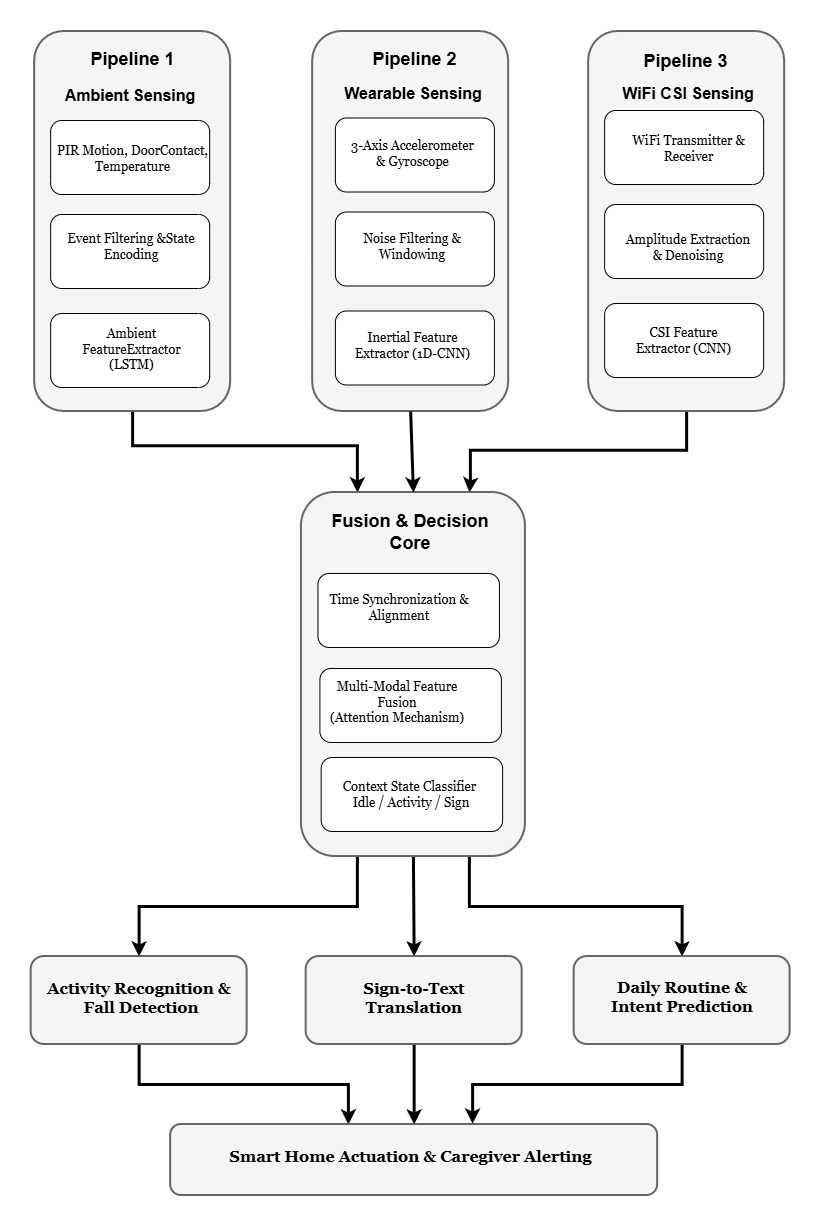
\includegraphics[
    width=0.88\textwidth,
    height=0.78\textheight,
    keepaspectratio
]{Arch_FYP.jpg}
\end{center}
\end{frame}


% =========================================================
% 8. SYSTEM EVOLUTION
% =========================================================

\begin{frame}{9. System Evolution: From Passive Capture to Controlled CSI}
\roone

\begin{columns}[T,totalwidth=\textwidth]

\column{0.45\textwidth}

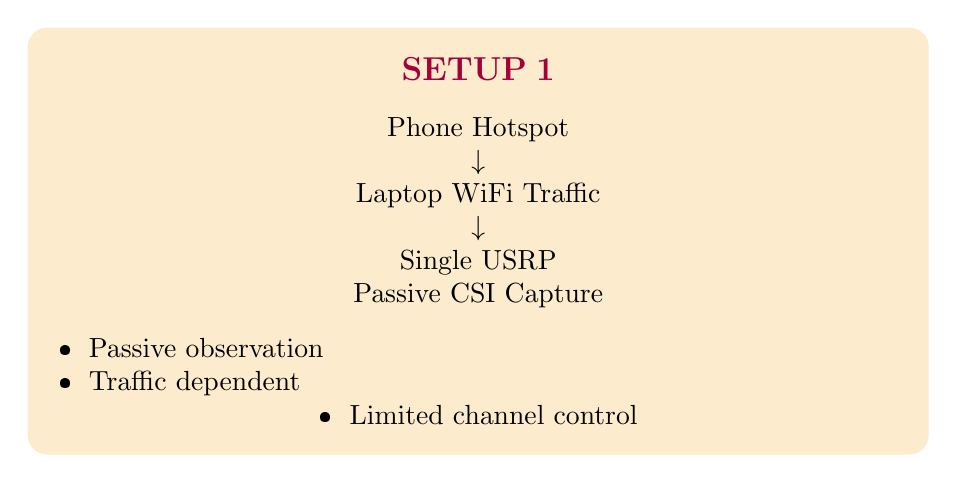
\begin{tikzpicture}
\node[
    rounded corners=7pt,
    fill=LightOrange,
    inner sep=11pt,
    text width=0.88\textwidth,
    align=center
] {
    {\large\bfseries\color{AmritaMaroon} SETUP 1}\\[8pt]

    Phone Hotspot\\
    $\downarrow$\\
    Laptop WiFi Traffic\\
    $\downarrow$\\
    Single USRP\\
    Passive CSI Capture\\[8pt]

    \raggedright
    \textbullet\; Passive observation\\
    \textbullet\; Traffic dependent\\
    \textbullet\; Limited channel control
};
\end{tikzpicture}

\column{0.08\textwidth}

\begin{center}
\vspace{1.8cm}
{\Huge $\Rightarrow$}
\end{center}

\column{0.45\textwidth}

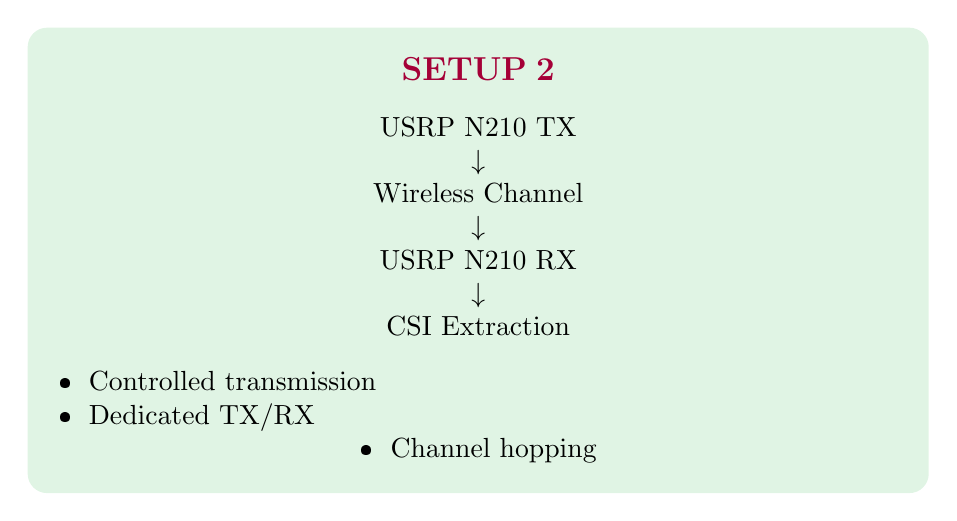
\begin{tikzpicture}
\node[
    rounded corners=7pt,
    fill=LightGreen,
    inner sep=11pt,
    text width=0.88\textwidth,
    align=center
] {
    {\large\bfseries\color{AmritaMaroon}SETUP 2}\\[8pt]

    USRP N210 TX\\
    $\downarrow$\\
    Wireless Channel\\
    $\downarrow$\\
    USRP N210 RX\\
    $\downarrow$\\
    CSI Extraction\\[8pt]

    \raggedright
    \textbullet\; Controlled transmission\\
    \textbullet\; Dedicated TX/RX\\
    \textbullet\; Channel hopping
};
\end{tikzpicture}

\end{columns}

\vspace{0.35cm}

\begin{center}
\textbf{\color{AmritaMaroon}Key change:}
From passive WiFi observation to a controlled SDR-based CSI platform.
\end{center}

\end{frame}


% =========================================================
% 15. CSI DATA
% =========================================================

\begin{frame}{10. CSI Data: From Channel Response to HAR Input}
\roone

\begin{center}

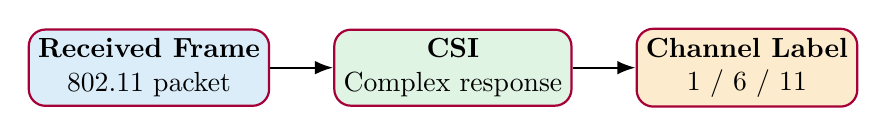
\begin{tikzpicture}[
    box/.style={
        rounded corners=6pt,
        minimum width=2.7cm,
        minimum height=0.78cm,
        align=center,
        draw=AmritaMaroon,
        thick
    },
    arr/.style={-{Latex},thick}
]

\node[box,fill=LightBlue] (frame)
{\textbf{Received Frame}\\802.11 packet};

\node[box,fill=LightGreen,right=0.8cm of frame] (csi)
{\textbf{CSI}\\Complex response};

\node[box,fill=LightOrange,right=0.8cm of csi] (label)
{\textbf{Channel Label}\\1 / 6 / 11};

\draw[arr] (frame)--(csi);
\draw[arr] (csi)--(label);

\end{tikzpicture}

\vspace{0.35cm}

\begin{columns}[T,totalwidth=\textwidth]

\column{0.48\textwidth}

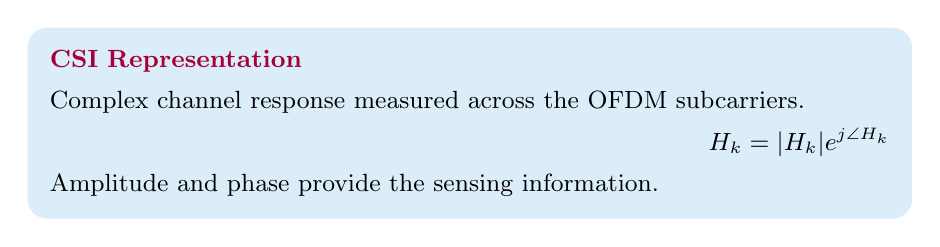
\begin{tikzpicture}
\node[
    rounded corners=7pt,
    fill=LightBlue,
    inner sep=8pt,
    text width=0.88\textwidth,
    align=left,
    font=\small
] {
\textbf{\color{AmritaMaroon}CSI Representation}\\[4pt]

Complex channel response measured across
the OFDM subcarriers.\\[4pt]

\hspace*{\fill}$H_k = |H_k|e^{j\angle H_k}$\hspace*{\fill}\\[4pt]

Amplitude and phase provide the sensing information.
};
\end{tikzpicture}

\column{0.48\textwidth}

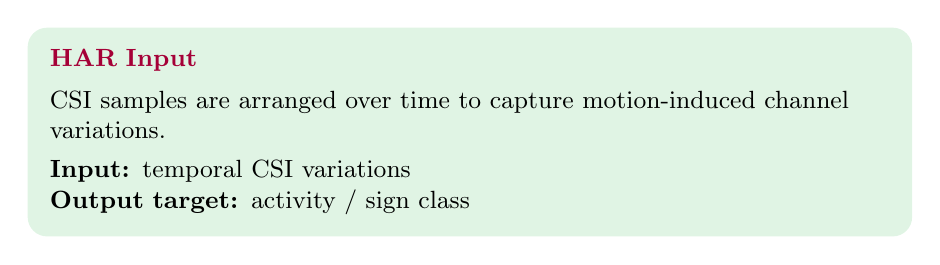
\begin{tikzpicture}
\node[
    rounded corners=7pt,
    fill=LightGreen,
    inner sep=8pt,
    text width=0.88\textwidth,
    align=left,
    font=\small
] {
\textbf{\color{AmritaMaroon}HAR Input}\\[4pt]

CSI samples are arranged over time to capture
motion-induced channel variations.

\vspace{3pt}

\textbf{Input:} temporal CSI variations\\
\textbf{Output target:} activity / sign class
};
\end{tikzpicture}

\end{columns}

\vspace{0.25cm}

{\small\textbf{\color{AmritaMaroon}Key result:}
Each CSI sample is associated with the active WiFi channel,
enabling channel-aware HAR analysis.}

\end{center}

\end{frame}

% =========================================================
% CSI MATHEMATICAL MODEL
% =========================================================

\begin{frame}{11. CSI Mathematical Model}
\roone

\vspace{0.2cm}
\begin{center}
    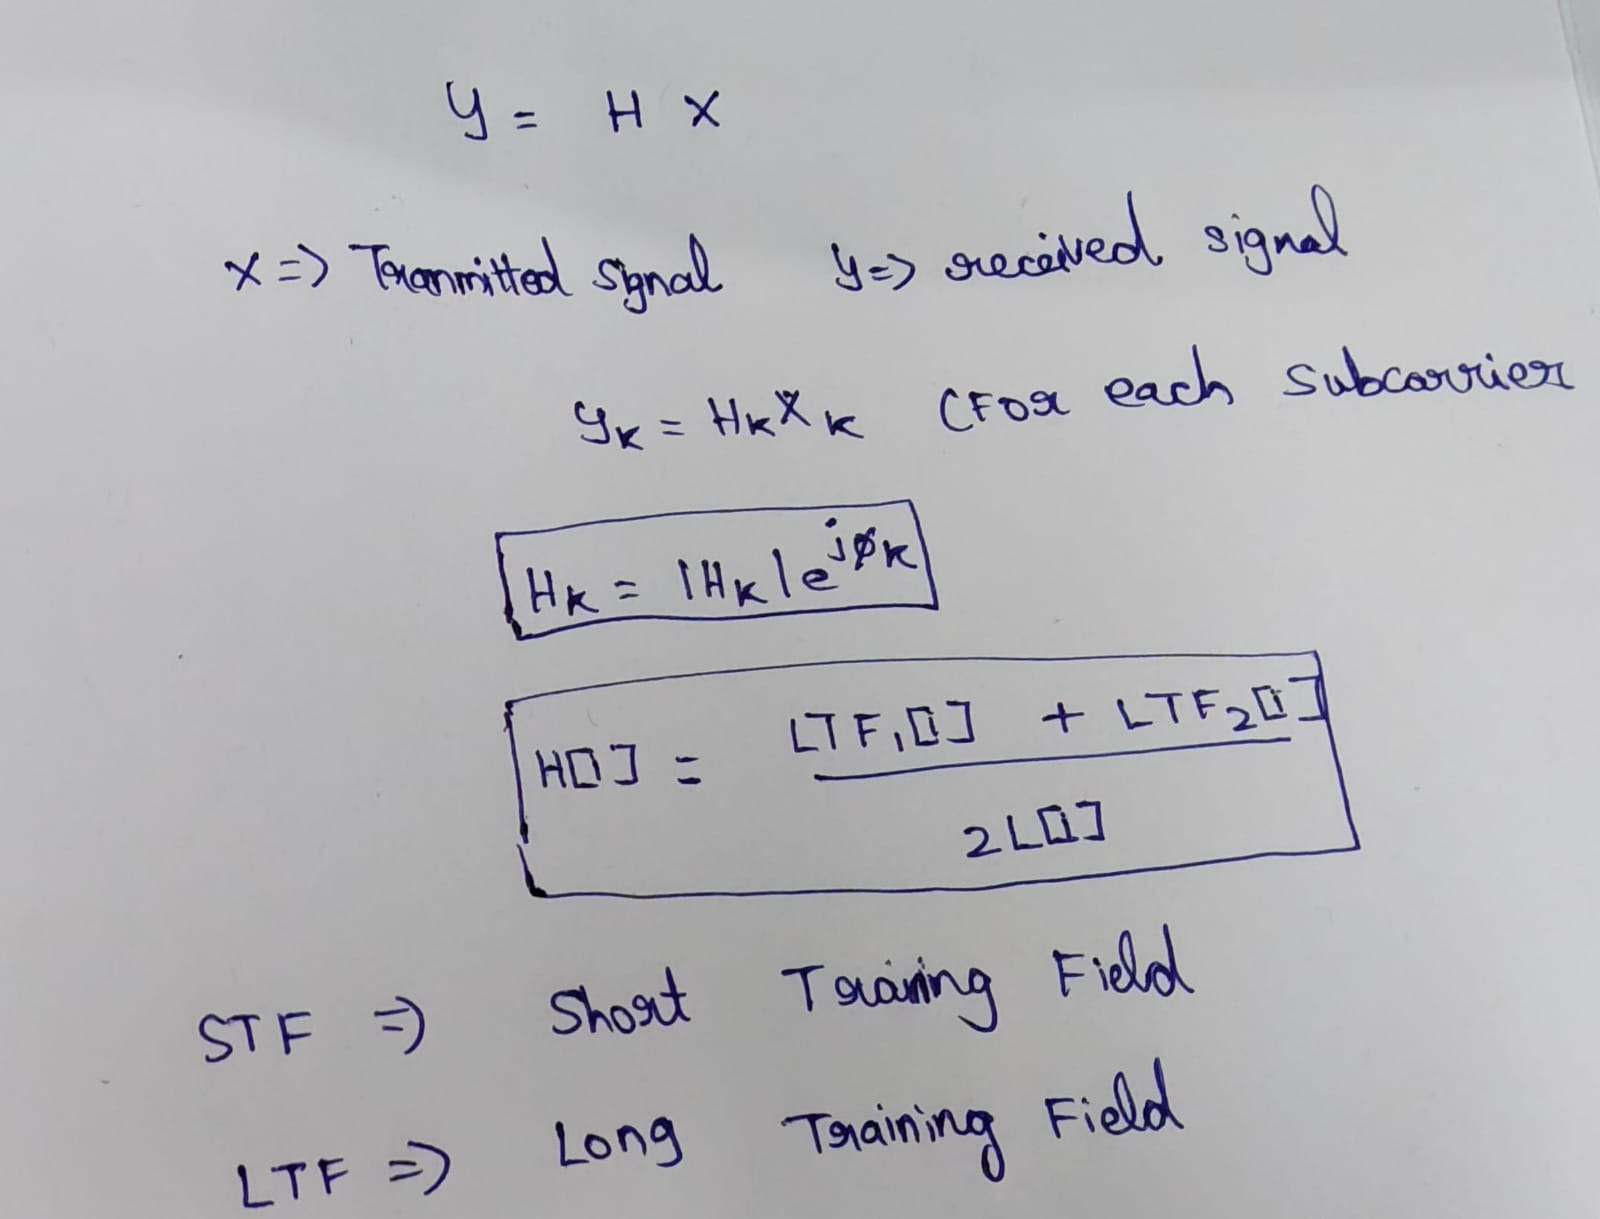
\includegraphics[width=0.85\textwidth,height=0.7\textheight,keepaspectratio]{csi_equations.jpeg}
\end{center}
\end{frame}


% =========================================================
% 12. CSI PROCESSING AND SOFTWARE ARCHITECTURE
% =========================================================

\begin{frame}{12. CSI Processing and Software Architecture}
\roone

\vspace{0.1cm}

\begin{center}

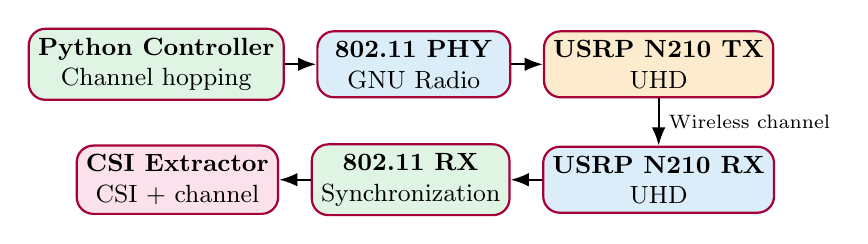
\begin{tikzpicture}[
    box/.style={
        rounded corners=6pt,
        minimum width=2.45cm,
        minimum height=0.6cm,
        align=center,
        draw=AmritaMaroon,
        thick,
        font=\small
    },
    arr/.style={-{Latex},thick}
]

\node[
    box,
    fill=LightGreen
] (controller)
{\textbf{Python Controller}\\Channel hopping};

\node[
    box,
    fill=LightBlue,
    right=0.4cm of controller
] (txphy)
{\textbf{802.11 PHY}\\GNU Radio};

\node[
    box,
    fill=LightOrange,
    right=0.4cm of txphy
] (txusrp)
{\textbf{USRP N210 TX}\\UHD};

\node[
    box,
    fill=LightBlue,
    below=0.6cm of txusrp
] (rxusrp)
{\textbf{USRP N210 RX}\\UHD};

\node[
    box,
    fill=LightGreen,
    left=0.4cm of rxusrp
] (sync)
{\textbf{802.11 RX}\\Synchronization};

\node[
    box,
    fill=LightPink,
    left=0.4cm of sync
] (csi)
{\textbf{CSI Extractor}\\CSI + channel};

\draw[arr] (controller)--(txphy);
\draw[arr] (txphy)--(txusrp);

\draw[arr] (txusrp) -- node[right,font=\scriptsize]
{Wireless channel} (rxusrp);

\draw[arr] (rxusrp)--(sync);
\draw[arr] (sync)--(csi);

\end{tikzpicture}

\vspace{0.2cm}

\begin{columns}[T,totalwidth=\textwidth]

\column{0.48\textwidth}

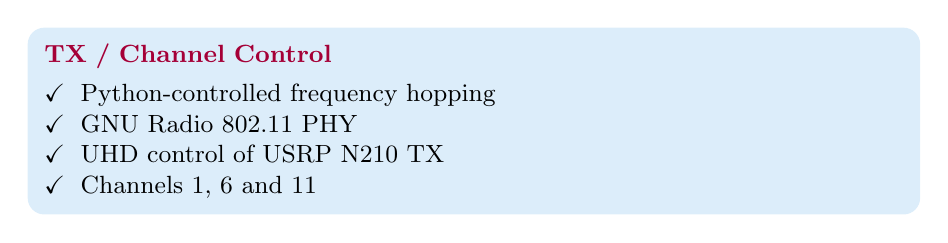
\begin{tikzpicture}
\node[
    rounded corners=6pt,
    fill=LightBlue,
    inner sep=6pt,
    text width=0.9\textwidth,
    align=left,
    font=\small
] {
\textbf{\color{AmritaMaroon}TX / Channel Control}\\[3pt]
$\checkmark$\; Python-controlled frequency hopping\\
$\checkmark$\; GNU Radio 802.11 PHY\\
$\checkmark$\; UHD control of USRP N210 TX\\
$\checkmark$\; Channels 1, 6 and 11
};
\end{tikzpicture}

\column{0.48\textwidth}

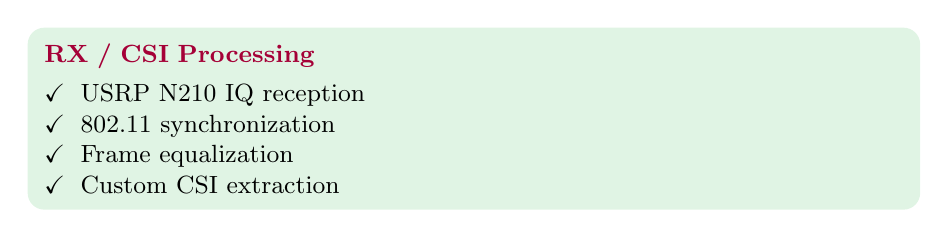
\begin{tikzpicture}
\node[
    rounded corners=6pt,
    fill=LightGreen,
    inner sep=6pt,
    text width=0.9\textwidth,
    align=left,
    font=\small
] {
\textbf{\color{AmritaMaroon}RX / CSI Processing}\\[3pt]
$\checkmark$\; USRP N210 IQ reception\\
$\checkmark$\; 802.11 synchronization\\
$\checkmark$\; Frame equalization\\
$\checkmark$\; Custom CSI extraction
};
\end{tikzpicture}

\end{columns}

\vspace{0.15cm}

{\small \textbf{\color{AmritaMaroon}Current output:}
CSI measurements associated with the active channel.}

\end{center}

\end{frame}



% =========================================================
% 9. CURRENT IMPLEMENTATION
% =========================================================

\begin{frame}{13. Current Implementation: Two-USRP CSI Setup}
\roone
\vspace{0.15cm}

\begin{center}


\begin{tikzpicture}[
    box/.style={
        rounded corners=6pt,
        minimum width=3.0cm,
        minimum height=0.9cm,
        align=center,
        draw=AmritaMaroon,
        thick
    },
    arr/.style={-{Latex},thick}
]

\node[box,fill=LightGreen] (tx)
{\textbf{USRP N210 TX}\\IEEE 802.11};

\node[box,fill=LightOrange,right=1.0cm of tx] (air)
{\textbf{Wireless Channel}\\Human motion};

\node[box,fill=LightBlue,right=1.0cm of air] (rx)
{\textbf{USRP N210 RX}\\IQ capture};

\draw[arr] (tx)--(air);
\draw[arr] (air)--(rx);

\end{tikzpicture}

\vspace{0.40cm}

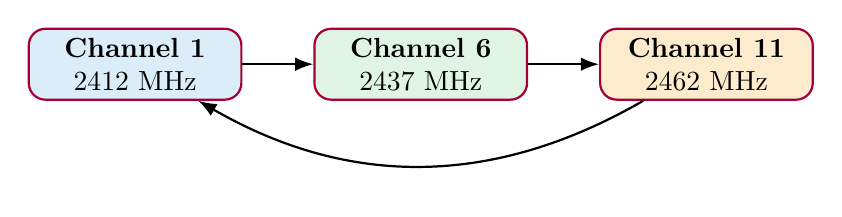
\begin{tikzpicture}[
    ch/.style={
        rounded corners=6pt,
        minimum width=2.7cm,
        minimum height=0.78cm,
        align=center,
        draw=AmritaMaroon,
        thick
    },
    arr/.style={-{Latex},thick}
]

\node[ch,fill=LightBlue] (c1)
{\textbf{Channel 1}\\2412 MHz};

\node[ch,fill=LightGreen,right=0.9cm of c1] (c6)
{\textbf{Channel 6}\\2437 MHz};

\node[ch,fill=LightOrange,right=0.9cm of c6] (c11)
{\textbf{Channel 11}\\2462 MHz};

\draw[arr] (c1)--(c6);
\draw[arr] (c6)--(c11);
\draw[arr] (c11) to[bend left=30] (c1);

\end{tikzpicture}

\vspace{0.20cm}

\begin{columns}[T,totalwidth=\textwidth]

\column{0.48\textwidth}

\begin{itemize}
    \item Controlled IEEE 802.11 transmission
    \item Dedicated SDR transmitter and receiver
\end{itemize}

\column{0.48\textwidth}

\begin{itemize}
    \item Current collection: fixed Channel 1 (2412 MHz)
    \item Hopping retained as an optional hardware capability
\end{itemize}

\end{columns}

\end{center}

\end{frame}


% =========================================================
% 10. CSI TRANSMISSION PIPELINE
% =========================================================

\begin{frame}{14. CSI Transmission Pipeline}
\roone

\begin{center}

\includegraphics[
    width=0.9\textwidth,
    height=4.5cm,
    keepaspectratio
]{tx_gnuradio.png}

\vspace{0.15cm}

\textbf{\color{AmritaMaroon}Key result:}

Network payloads are encoded into 802.11 WiFi frames and
transmitted via USRP to enable continuous channel measurement.

\end{center}

\end{frame}


% =========================================================
% 11. CSI ACQUISITION PIPELINE
% =========================================================

\begin{frame}{15. CSI Acquisition Pipeline}
\roone
\begin{center}
    \includegraphics[width=0.82\textwidth, height=0.68\textheight, keepaspectratio]{rx_gnuradio.png}

    \vspace{0.15cm}
    {\footnotesize
    \textbf{\color{AmritaMaroon}Key result:}
    Received WiFi frames are converted into CSI measurements
    for subsequent HAR analysis.
    }
\end{center}
\end{frame}

% =========================================================
% 16. USRP N210 HARDWARE
% =========================================================
\begin{frame}{16. USRP N210 Hardware}
\roone

\begin{columns}[T,totalwidth=\textwidth]


% ---------- Left column ----------
\column{0.48\textwidth}
\centering

\begin{minipage}[t][4.0cm][c]{\linewidth}
    \centering
    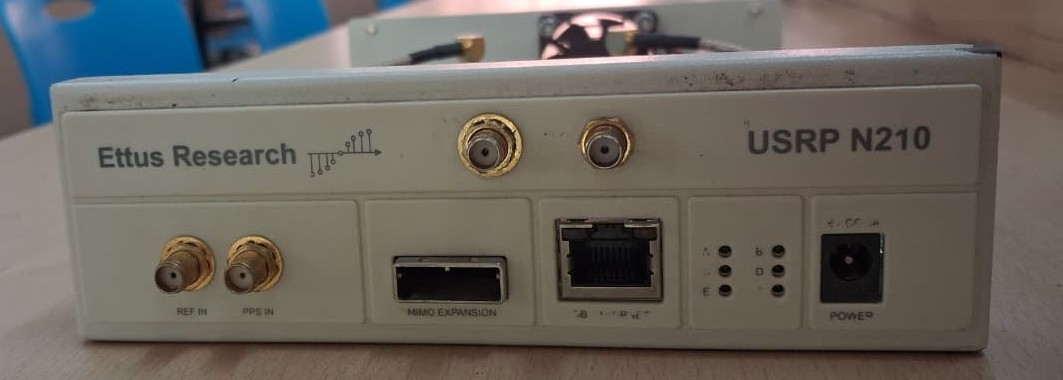
\includegraphics[
        width=\linewidth,
        height=3.8cm,
        keepaspectratio
    ]{USRP_IMAGE_1.jpeg}
\end{minipage}

\vspace{0.08cm}

\parbox[t][1.0cm][t]{\linewidth}{%
    \centering
    \scriptsize
    \color{AmritaDark}
    \textit{Front panel --- RF, MIMO expansion,\\
    Gigabit Ethernet, PPS/REF sync}
}

% ---------- Right column ----------
\column{0.48\textwidth}
\centering

\begin{minipage}[t][4.0cm][c]{\linewidth}
    \centering
    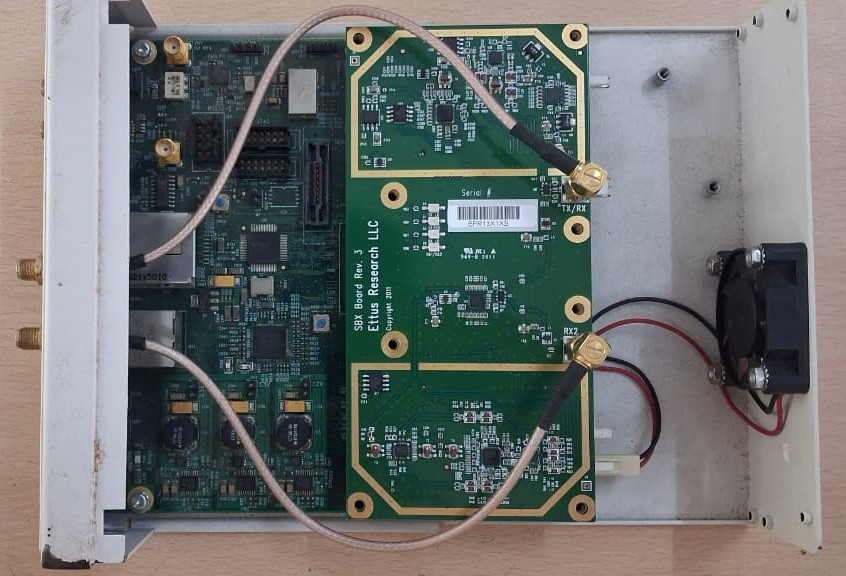
\includegraphics[
        width=\linewidth,
        height=3.8cm,
        keepaspectratio
    ]{USRP_IMAGE_2.jpeg}
\end{minipage}

\vspace{0.08cm}

\parbox[t][1.0cm][t]{\linewidth}{%
    \centering
    \scriptsize
    \color{AmritaDark}
    \textit{Internal SBX daughterboard --- TX/RX\\
    and RX2 RF front-end}
}

\end{columns}

\vspace{0.05cm}

% ---------- Summary box ----------
\begin{center}
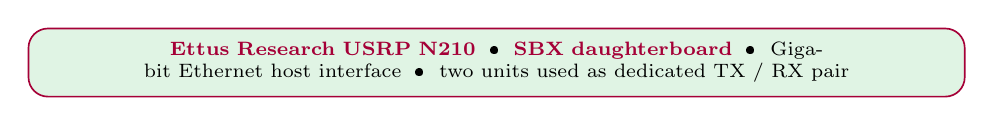
\begin{tikzpicture}
\node[
    rounded corners=7pt,
    fill=LightGreen,
    draw=AmritaMaroon,
    line width=0.6pt,
    inner xsep=7pt,
    inner ysep=5pt,
    text width=0.94\textwidth,
    align=center,
    font=\scriptsize
] {%
    \textbf{\color{AmritaMaroon}Ettus Research USRP N210}
    \;\textbullet\;
    \textbf{\color{AmritaMaroon}SBX daughterboard}
    \;\textbullet\;
    Gigabit Ethernet host interface
    \;\textbullet\;
    two units used as dedicated TX / RX pair
};
\end{tikzpicture}
\end{center}

\end{frame}

% =========================================================
% 14. ACTIVE VS. PASSIVE CSI SENSING
% =========================================================

\begin{frame}{17. Active vs.\ Passive CSI Sensing}
\roone

\vspace{-0.05cm}

\begin{columns}[T,totalwidth=\textwidth]

\column{0.48\textwidth}

\begin{center}
{\bfseries\color{AmritaMaroon} Passive Sensing}
\end{center}

\vspace{0.08cm}

\begin{center}
\begin{minipage}[c][2.7cm][c]{0.95\linewidth}
\centering
\includegraphics[width=\linewidth,height=2.7cm,keepaspectratio]{Passive.jpeg}
\end{minipage}
\end{center}

\vspace{0.12cm}

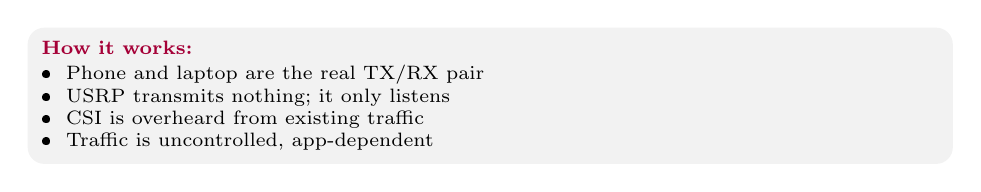
\begin{tikzpicture}
\node[
    rounded corners=6pt,
    fill=LightGray,
    inner sep=5pt,
    text width=0.94\textwidth,
    align=left,
    font=\scriptsize
] {
\textbf{\color{AmritaMaroon}How it works:}\\[1pt]
\raggedright
\textbullet\; Phone and laptop are the real TX/RX pair\\
\textbullet\; USRP transmits nothing; it only listens\\
\textbullet\; CSI is overheard from existing traffic\\
\textbullet\; Traffic is uncontrolled, app-dependent
};
\end{tikzpicture}

\column{0.48\textwidth}

\begin{center}
{\bfseries\color{AmritaMaroon} Active Sensing}
\end{center}

\vspace{0.08cm}

\begin{center}
\begin{minipage}[c][2.7cm][c]{0.95\linewidth}
\centering
\includegraphics[width=\linewidth,height=2.7cm,keepaspectratio]{Active.jpeg}
\end{minipage}
\end{center}

\vspace{0.12cm}

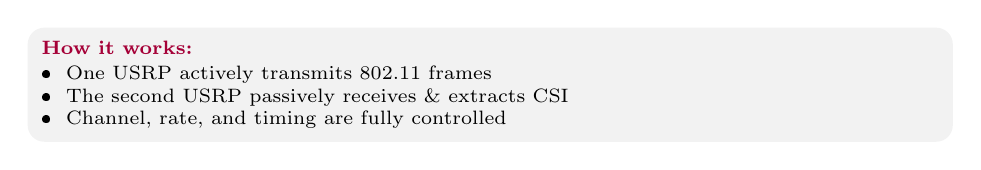
\begin{tikzpicture}
\node[
    rounded corners=6pt,
    fill=LightGray,
    inner sep=5pt,
    text width=0.94\textwidth,
    align=left,
    font=\scriptsize
] {
\textbf{\color{AmritaMaroon}How it works:}\\[1pt]
\raggedright
\textbullet\; One USRP actively transmits 802.11 frames\\
\textbullet\; The second USRP passively receives \& extracts CSI\\
\textbullet\; Channel, rate, and timing are fully controlled\\
};
\end{tikzpicture}

\end{columns}

\vspace{0.15cm}

\begin{center}
\small
\textbf{\color{AmritaMaroon}Key Insight:}
Passive sensing eavesdrops on someone else's traffic; active sensing uses a dedicated TX--RX pair for reliable, repeatable CSI.
\end{center}

\end{frame}


% =========================================================
% 17. DATASET 1: ACTION VS NO-ACTION
% =========================================================

\begin{frame}{18. Dataset 1: Action vs.\ No-Action}
\roone

\begin{columns}[T,totalwidth=\textwidth]

% ---------- LEFT: classes and volume ----------
\column{0.42\textwidth}

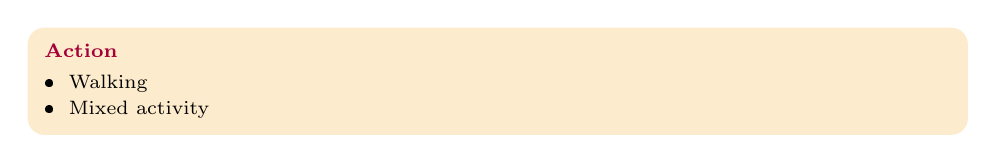
\begin{tikzpicture}
\node[
    rounded corners=6pt,
    fill=LightOrange,
    inner sep=6pt,
    text width=0.95\textwidth,
    align=left,
    font=\scriptsize
] {
\textbf{\color{AmritaMaroon}Action}\\[3pt]
\textbullet\; Walking\\[1.5pt]
\textbullet\; Mixed activity
};
\end{tikzpicture}

\vspace{0.12cm}

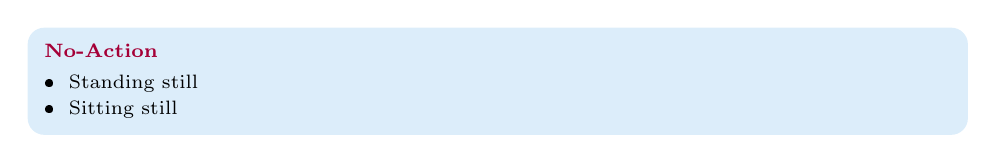
\begin{tikzpicture}
\node[
    rounded corners=6pt,
    fill=LightBlue,
    inner sep=6pt,
    text width=0.95\textwidth,
    align=left,
    font=\scriptsize
] {
\textbf{\color{AmritaMaroon}No-Action}\\[3pt]
\textbullet\; Standing still\\[1.5pt]
\textbullet\; Sitting still
};
\end{tikzpicture}

\vspace{0.12cm}

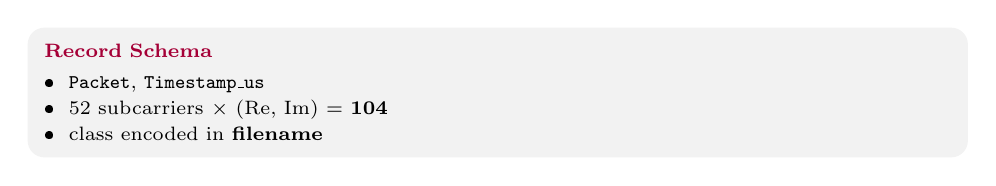
\begin{tikzpicture}
\node[
    rounded corners=6pt,
    fill=LightGray,
    inner sep=6pt,
    text width=0.95\textwidth,
    align=left,
    font=\scriptsize
] {
\textbf{\color{AmritaMaroon}Record Schema}\\[3pt]
\textbullet\; \texttt{Packet}, \texttt{Timestamp\_us}\\[1.5pt]
\textbullet\; 52 subcarriers $\times$ (Re, Im) $=$ \textbf{104}\\[1.5pt]
\textbullet\; class encoded in \textbf{filename}
};
\end{tikzpicture}

% ---------- RIGHT: dataset screenshot ----------
\column{0.56\textwidth}

\centering

\includegraphics[
    width=0.95\linewidth,
    height=3.75cm,
    keepaspectratio
]{dataset_1_pic.png}

\vspace{0.08cm}

{\scriptsize\color{AmritaDark}\textit{Raw CSI capture --- one row per decoded
802.11 packet}}

\end{columns}

\vspace{0.10cm}

\begin{center}
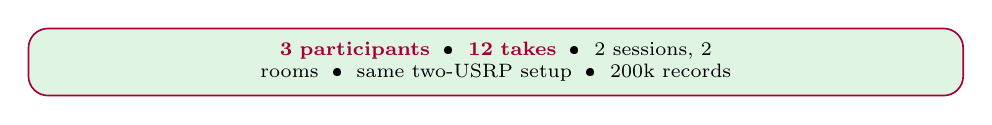
\begin{tikzpicture}
\node[
    rounded corners=7pt,
    fill=LightGreen,
    draw=AmritaMaroon,
    line width=0.6pt,
    inner sep=5pt,
    text width=0.95\textwidth,
    align=center,
    font=\scriptsize
] {
\textbf{\color{AmritaMaroon}3 participants}
\;\textbullet\;
\textbf{\color{AmritaMaroon}12 takes}
\;\textbullet\;
2 sessions, 2 rooms
\;\textbullet\;
same two-USRP setup
\;\textbullet\;
200k records
};

\end{tikzpicture}

\end{center}

\end{frame}


% =========================================================
% 19. DATA COLLECTION: WALKING & STANDING
% =========================================================

\begin{frame}{19. Data Collection: Walking \& Standing}
\roone

\vspace{-0.05cm}

% ---------------- ROW 1 : WALKING ----------------
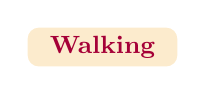
\begin{tikzpicture}
\node[rounded corners=4pt,fill=LightOrange,inner xsep=8pt,inner ysep=3pt]
{\small\bfseries\color{AmritaMaroon}Walking};
\end{tikzpicture}
{\scriptsize\color{AmritaDark}\;\;action take \textperiodcentered\ Amrith \textperiodcentered\ Room A}

\vspace{0.08cm}

\begin{columns}[c,totalwidth=\textwidth]
\column{0.62\textwidth}
\centering
\includegraphics[height=2.5cm,keepaspectratio]{ppt_images/graph_walk.png}
\column{0.36\textwidth}
\centering
\includegraphics[height=2.5cm,keepaspectratio]{ppt_images/person_walk.png}
\end{columns}

\vspace{0.22cm}

% ---------------- ROW 2 : STANDING ----------------
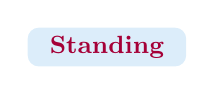
\begin{tikzpicture}
\node[rounded corners=4pt,fill=LightBlue,inner xsep=8pt,inner ysep=3pt]
{\small\bfseries\color{AmritaMaroon}Standing};
\end{tikzpicture}
{\scriptsize\color{AmritaDark}\;\;no-action take \textperiodcentered\ Rishiikesh \textperiodcentered\ Room A}

\vspace{0.08cm}

\begin{columns}[c,totalwidth=\textwidth]
\column{0.62\textwidth}
\centering
\includegraphics[height=2.5cm,keepaspectratio]{ppt_images/graph_stand.png}
\column{0.36\textwidth}
\centering
\includegraphics[height=2.5cm,keepaspectratio]{ppt_images/person_stand.png}
\end{columns}

\end{frame}


% =========================================================
% 20. DATA COLLECTION: SITTING & MIXED ACTIVITY
% =========================================================

\begin{frame}{20. Data Collection: Sitting \& Mixed Activity}
\roone

\vspace{-0.05cm}

% ---------------- ROW 1 : SITTING ----------------
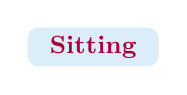
\begin{tikzpicture}
\node[rounded corners=4pt,fill=LightBlue,inner xsep=8pt,inner ysep=3pt]
{\small\bfseries\color{AmritaMaroon}Sitting};
\end{tikzpicture}
{\scriptsize\color{AmritaDark}\;\;no-action take \textperiodcentered\ Rishiikesh \textperiodcentered\ Room A}

\vspace{0.08cm}

\begin{columns}[c,totalwidth=\textwidth]
\column{0.62\textwidth}
\centering
\includegraphics[height=2.5cm,keepaspectratio]{ppt_images/graph_sit.png}
\column{0.36\textwidth}
\centering
\includegraphics[height=2.5cm,keepaspectratio]{ppt_images/person_sit.png}
\end{columns}

\vspace{0.22cm}

% ---------------- ROW 2 : MIXED ACTIVITY ----------------
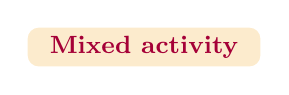
\begin{tikzpicture}
\node[rounded corners=4pt,fill=LightOrange,inner xsep=8pt,inner ysep=3pt]
{\small\bfseries\color{AmritaMaroon}Mixed activity};
\end{tikzpicture}
{\scriptsize\color{AmritaDark}\;\;action take \textperiodcentered\ Gowreesh \textperiodcentered\ Room B}

\vspace{0.08cm}

\begin{columns}[c,totalwidth=\textwidth]
\column{0.62\textwidth}
\centering
\includegraphics[height=2.5cm,keepaspectratio]{ppt_images/graph_mixed.png}
\column{0.36\textwidth}
\centering
\includegraphics[height=2.5cm,keepaspectratio]{ppt_images/person_mixed.png}
\end{columns}

\end{frame}


% =========================================================
% 21. DATASET STRUCTURE
% =========================================================
\begin{frame}{21. Current Dataset: Collection and Coverage}
\roone
\begin{columns}[T,onlytextwidth]
\column{0.56\textwidth}
{\small\textbf{\color{AmritaMaroon}5 people \quad 25 kept recordings \quad 2,050,030 raw rows}}
\vspace{0.13cm}

\scriptsize
\renewcommand{\arraystretch}{1.32}
\begin{tabular}{@{}lrr@{}}
\toprule
\textbf{Recording block} & \textbf{Files} & \textbf{CSI rows}\\
\midrule
Actions: main block & 5 & 844,426\\
Actions: seated & 2 & 173,297\\
Signs: standing & 5 & 457,408\\
Signs: seated & 2 & 127,209\\
Interleaved stories & 5 & 354,465\\
Still-person baselines & 3 & 54,094\\
Empty-room checks & 3 & 39,131\\
\midrule
\textbf{Total collected} & \textbf{25} & \textbf{2,050,030}\\
\bottomrule
\end{tabular}
\vspace{0.15cm}

\implnote{Model input: \textbf{22 files / 2,010,899 rows}.
Recording totals include rest/ready; empty-room files are QC only.}
\column{0.41\textwidth}
\centering
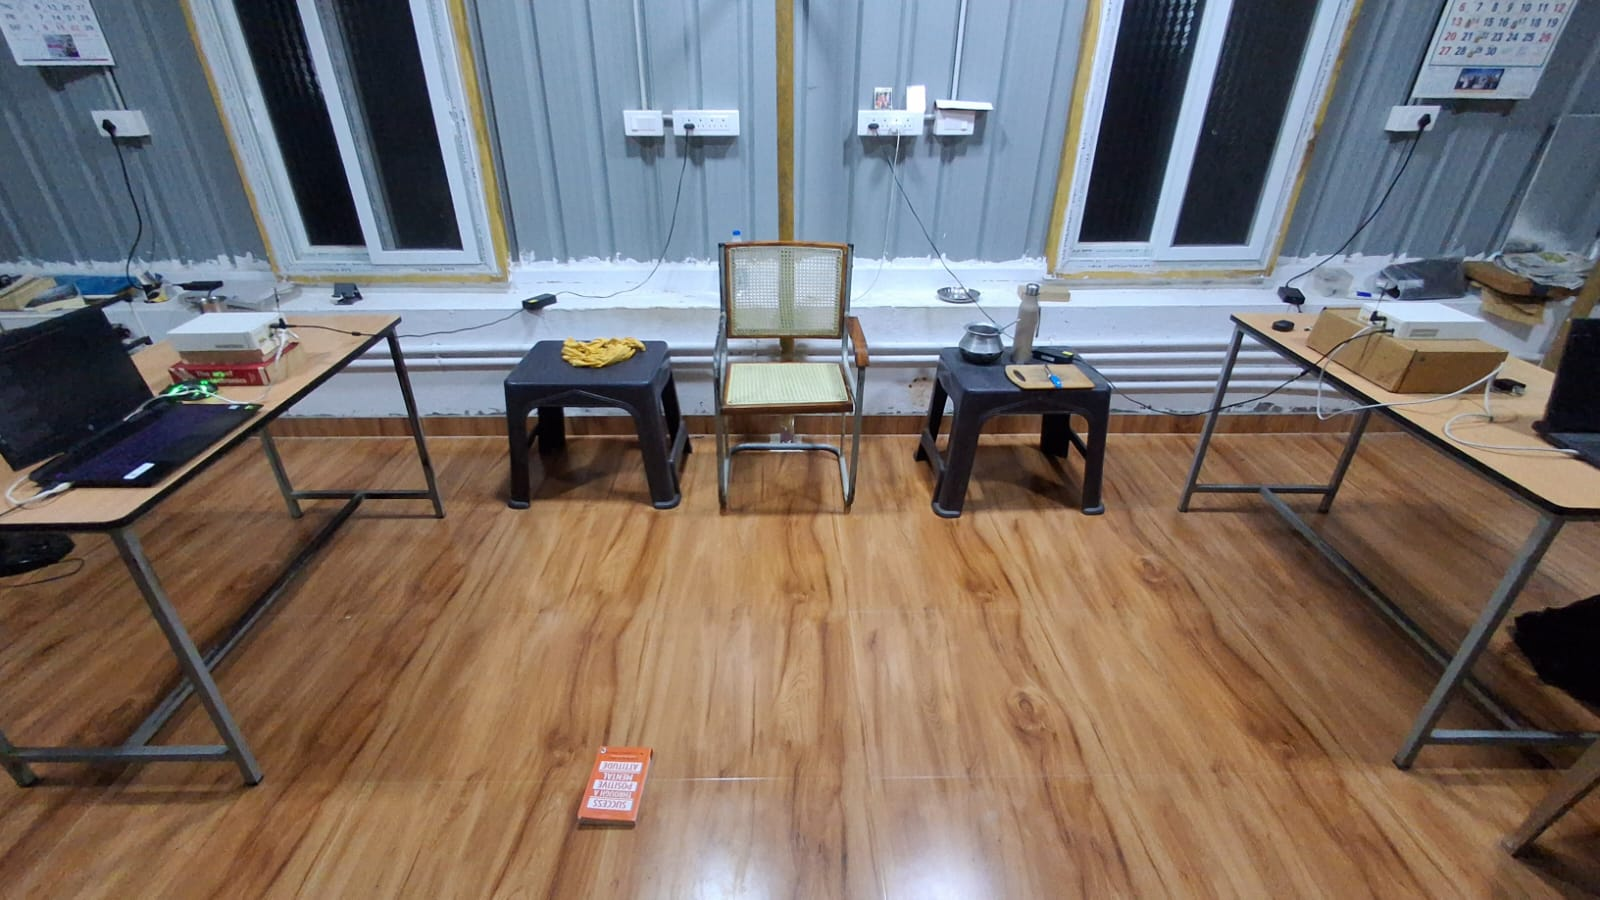
\includegraphics[width=\linewidth,height=2.45cm,keepaspectratio]{current_impl/media/collection_setup.jpeg}
\vspace{0.16cm}

\raggedright\footnotesize
\textbf{\color{AmritaMaroon}Collection conditions}\\[3pt]
Two USRP N210s; Channel 1, 2412 MHz.\\[3pt]
Same room and antenna positions.\\[3pt]
One active participant at a time.\\[3pt]
P4/P5 add seated blocks and cooking actions.
\end{columns}
\end{frame}


% =========================================================
% 18. DATASET: CLASSES AND PARTICIPANTS
% =========================================================

\begin{frame}{22. Current Dataset: Actions and Signs}
\roone
\begin{columns}[T,onlytextwidth]
\column{0.49\textwidth}
\raggedright
{\small\textbf{\color{AmritaMaroon}12 action labels}}\\[5pt]
\footnotesize
\renewcommand{\arraystretch}{1.16}
\begin{tabular}{@{}ll@{}}
Walk & Sit--stand\\
Pick up & Light switch\\
Drink & Answer phone\\
Eat & Wipe table\\
TV remote & Fall\\
Chop food & Stir pot
\end{tabular}
\vspace{0.14cm}

\implnote{628 isolated trials. P4/P5 add chop/stir and seven seated action types.}
\column{0.49\textwidth}
\raggedright
{\small\textbf{\color{AmritaMaroon}14 sign labels}}\\[5pt]
\footnotesize
\renewcommand{\arraystretch}{1.16}
\begin{tabular}{@{}ll@{}}
HELLO & THANKYOU\\
LAMP & FAN\\
TELEVISION & COOK\\
WATER & HOT\\
HUNGRY & TOILET\\
CALL & HELP\\
PAIN & ACCIDENT
\end{tabular}
\vspace{0.12cm}

\implnote{490 trials: 350 standing (P1--P5) + 140 seated (P4/P5).}
\end{columns}
\end{frame}



\begin{frame}{23. Current Dataset: Recording Demonstration}
\roone
\begin{columns}[T,onlytextwidth]
\column{0.485\textwidth}
\centering
{\small\textbf{\color{AmritaMaroon}Standing collection excerpt}}\par
\vspace{0.16cm}
\implclip{collection_action_pickup}{3.20cm}\par
\vspace{0.15cm}
{\footnotesize Standing participant within the collection area.\par}
\column{0.485\textwidth}
\centering
{\small\textbf{\color{AmritaMaroon}Seated collection excerpt}}\par
\vspace{0.16cm}
\implclip{collection_sign_cook_seated}{3.20cm}\par
\vspace{0.15cm}
{\footnotesize Seated posture and hand movement during recording.\par}
\end{columns}
\vspace{0.18cm}
\implnote{Short excerpts from the recorded collection videos. The label files define the action/sign classes and time intervals.}
\end{frame}

\begin{frame}{24. Current Dataset: Interleaved Stories}
\roonefour
\begin{columns}[T,onlytextwidth]
\column{0.62\textwidth}
\scriptsize
\renewcommand{\arraystretch}{1.35}
\begin{tabular}{@{}>{\raggedright\arraybackslash}p{1.35cm}>{\raggedright\arraybackslash}p{6.9cm}@{}}
\toprule
\textbf{Template} & \textbf{Recorded sequence / context}\\
\midrule
M-SEQ: meal & Walk, light switch, sit--stand, eat/drink; HELLO, HUNGRY, COOK, HOT, WATER, THANKYOU. P4/P5 add chop/stir.\\
T-SEQ: TV & Walk, sit--stand, TV remote, phone; HELLO, TELEVISION, HOT, LAMP, CALL, TOILET; stand and walk out.\\
C-SEQ: clean / fall & Walk, wipe, pick up; FAN, HELP; walk and fall; HELP, PAIN, ACCIDENT, CALL on the mattress.\\
S-SEQ: seated & Wipe, chop, stir, eat, drink; HELLO, HUNGRY, COOK, HOT, WATER, HELP, THANKYOU. P4/P5 only.\\
\bottomrule
\end{tabular}
\vspace{0.14cm}

\implnote{Each available template was repeated twice per person:
\textbf{34 runs / 416 labelled steps} = 208 actions + 208 signs.}
\column{0.35\textwidth}
\centering
\implclip{collection_story_meal}{2.30cm}
\par\vspace{0.10cm}{\scriptsize Story recording excerpt\par}
\vspace{0.12cm}

\raggedright\footnotesize
\textbf{\color{AmritaMaroon}Why stories matter}\\[4pt]
Actions and signs share one recording.\\[4pt]
HOT during a meal and HOT while watching TV have different intended responses.
\end{columns}
\end{frame}


\begin{frame}{25. Current Dataset: CSI Rows and Annotations}
\roone
\begin{center}
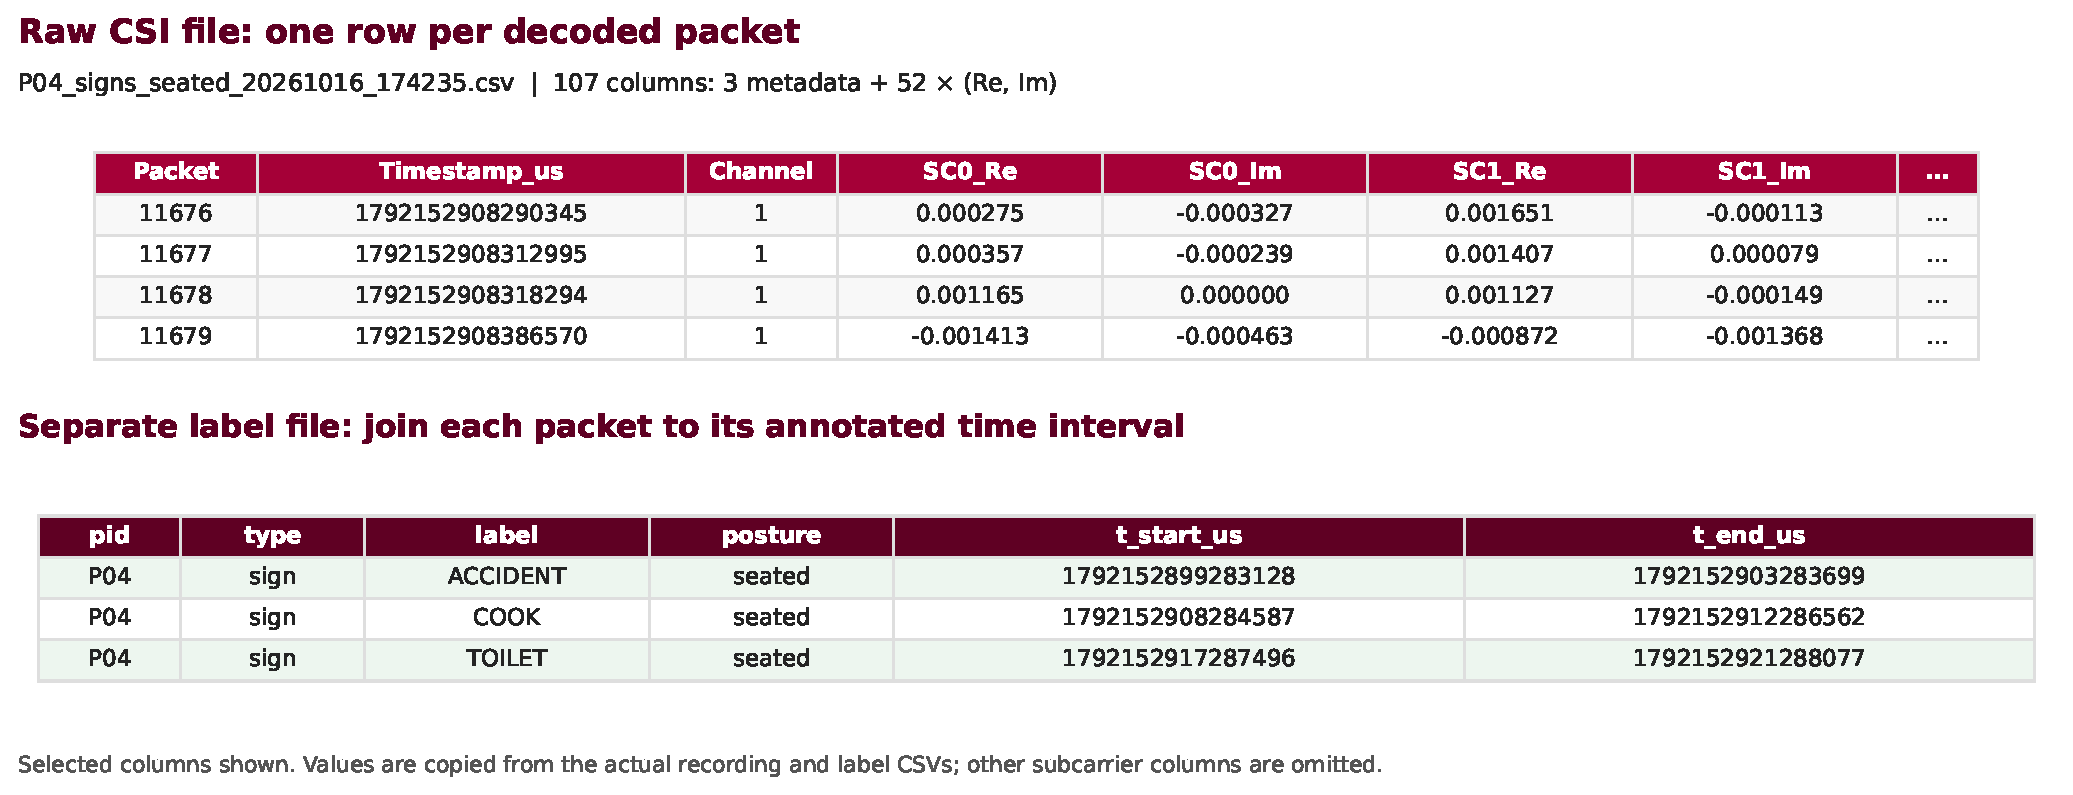
\includegraphics[width=0.97\linewidth,height=4.55cm,keepaspectratio]{current_impl/dataset_excerpt.pdf}
\end{center}
\vspace{-0.08cm}
\implnote{Actual CSV excerpt, selected columns. Raw rows contain packet/time/channel and complex CSI;
the separate label file supplies participant, type, label, posture and time boundaries.
Labels come from the collection cues/key presses; video alignment is not yet verified.}
\end{frame}


\begin{frame}{26. Current Dataset: Recording Rows per Class}
\roone
\begin{columns}[T,onlytextwidth]
\column{0.49\textwidth}
{\small\textbf{\color{AmritaMaroon}Actions}}\\[4pt]
\fontsize{7}{8.1}\selectfont\renewcommand{\arraystretch}{0.94}
\begin{tabular}{@{}lrr@{}}\toprule
\textbf{Class} & \textbf{Trials} & \textbf{Raw rows}\\\midrule
Answer phone & 67 & 46,741\\
Chop food & 40 & 25,679\\
Drink & 67 & 46,554\\
Eat & 67 & 46,401\\
Fall & 23 & 16,512\\
Light switch & 48 & 23,817\\
Pick up & 48 & 35,094\\
Sit--stand & 48 & 33,576\\
Stir pot & 40 & 25,174\\
TV remote & 67 & 39,134\\
Walk & 46 & 33,371\\
Wipe table & 67 & 44,783\\
\midrule\textbf{Total} & \textbf{628} & \textbf{416,836}\\
\bottomrule\end{tabular}
\column{0.49\textwidth}
{\small\textbf{\color{AmritaMaroon}Signs}}\\[4pt]
\fontsize{7}{8.1}\selectfont\renewcommand{\arraystretch}{0.94}
\begin{tabular}{@{}lrr@{}}\toprule
\textbf{Class} & \textbf{Trials} & \textbf{Raw rows}\\\midrule
ACCIDENT & 35 & 15,864\\
CALL & 35 & 15,815\\
COOK & 35 & 15,792\\
FAN & 35 & 15,956\\
HELLO & 35 & 16,019\\
HELP & 35 & 15,782\\
HOT & 35 & 16,097\\
HUNGRY & 35 & 16,140\\
LAMP & 35 & 15,689\\
PAIN & 35 & 16,051\\
TELEVISION & 35 & 15,641\\
THANKYOU & 35 & 15,697\\
TOILET & 35 & 15,875\\
WATER & 35 & 16,152\\
\midrule\textbf{Total} & \textbf{490} & \textbf{222,570}\\
\bottomrule\end{tabular}
\end{columns}
\vspace{0.10cm}
\implnote{Raw packets inside fully covered isolated label intervals; rest/ready and story steps excluded.
Partial P2 trials excluded. Chop/stir: P4/P5 only.}
\end{frame}

% =========================================================
% MULTI-MODAL EXTENSION: WEARABLE FALL DETECTION
% =========================================================

\begin{frame}{27. Multi-Modal Extension: Wearable Fall Detection}
\rofour
\vspace{-0.12cm}

\begin{center}
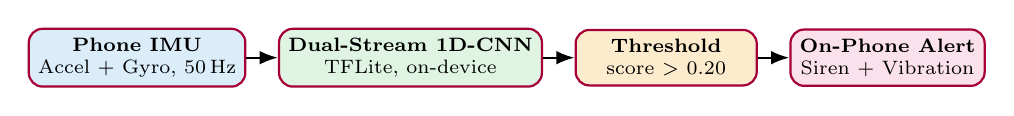
\begin{tikzpicture}[
    box/.style={
        rounded corners=5pt,
        minimum width=2.3cm,
        minimum height=0.6cm,
        align=center,
        draw=AmritaMaroon,
        thick,
        font=\scriptsize
    },
    arr/.style={-{Latex},thick}
]
\node[box,fill=LightBlue] (imu)
{\textbf{Phone IMU}\\Accel + Gyro, 50\,Hz};

\node[box,fill=LightGreen,right=0.4cm of imu] (cnn)
{\textbf{Dual-Stream 1D-CNN}\\TFLite, on-device};

\node[box,fill=LightOrange,right=0.4cm of cnn] (th)
{\textbf{Threshold}\\score $>$ 0.20};

\node[box,fill=LightPink,right=0.4cm of th] (alert)
{\textbf{On-Phone Alert}\\Siren + Vibration};

\draw[arr] (imu)--(cnn);
\draw[arr] (cnn)--(th);
\draw[arr] (th)--(alert);
\end{tikzpicture}
\end{center}

\vspace{0.1cm}

\begin{columns}[T,totalwidth=\textwidth]

\column{0.48\textwidth}

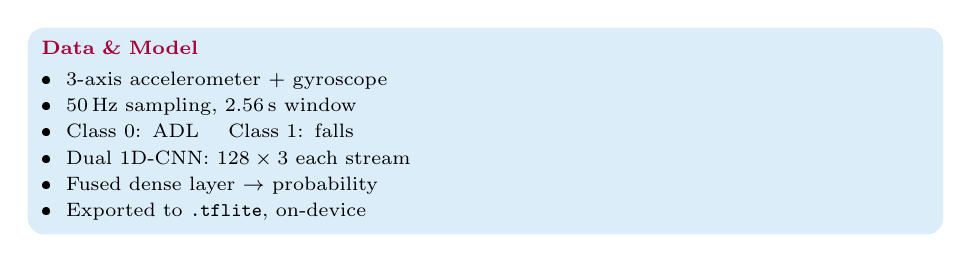
\begin{tikzpicture}
\node[
    rounded corners=6pt,
    fill=LightBlue,
    inner sep=5pt,
    text width=0.93\textwidth,
    align=left,
    font=\scriptsize
] {
\textbf{\color{AmritaMaroon}Data \& Model}\\[3pt]
\textbullet\; 3-axis accelerometer + gyroscope\\[1.5pt]
\textbullet\; 50\,Hz sampling, 2.56\,s window\\[1.5pt]
\textbullet\; Class 0: ADL \quad Class 1: falls\\[1.5pt]
\textbullet\; Dual 1D-CNN: $128\times3$ each stream\\[1.5pt]
\textbullet\; Fused dense layer $\rightarrow$ probability\\[1.5pt]
\textbullet\; Exported to \texttt{.tflite}, on-device
};
\end{tikzpicture}

\column{0.48\textwidth}

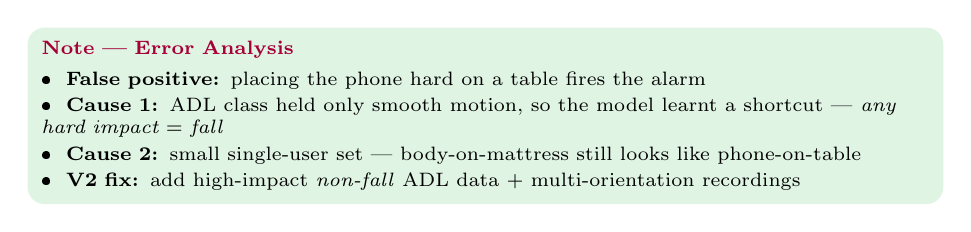
\begin{tikzpicture}
\node[
    rounded corners=6pt,
    fill=LightGreen,
    inner sep=5pt,
    text width=0.93\textwidth,
    align=left,
    font=\scriptsize
] {
\textbf{\color{AmritaMaroon}Note --- Error Analysis}\\[3pt]
\textbullet\; \textbf{False positive:} placing the phone hard on a table fires the alarm\\[1.5pt]
\textbullet\; \textbf{Cause 1:} ADL class held only smooth motion, so the model learnt a shortcut --- \textit{any hard impact $=$ fall}\\[1.5pt]
\textbullet\; \textbf{Cause 2:} small single-user set --- body-on-mattress still looks like phone-on-table\\[1.5pt]
\textbullet\; \textbf{V2 fix:} add high-impact \emph{non-fall} ADL data + multi-orientation recordings
};
\end{tikzpicture}

\end{columns}

\vspace{0.12cm}

\begin{center}
{\scriptsize
\textbf{\color{AmritaMaroon}Result:} ADL $4.8\times10^{-4}$ vs.\ fall $0.29$ --- a $\approx$\textbf{600$\times$} relative spike;
edge threshold set empirically at \textbf{0.20}
}
\end{center}

\end{frame}


% =========================================================
% MODEL ARCHITECTURE & METHODOLOGY
% =========================================================

\begin{frame}{28. Earlier Pilot: Binary Action Model}
\roone

\vspace{0.2cm}

\begin{columns}[T,onlytextwidth]

\column{0.62\textwidth}

\begin{center}

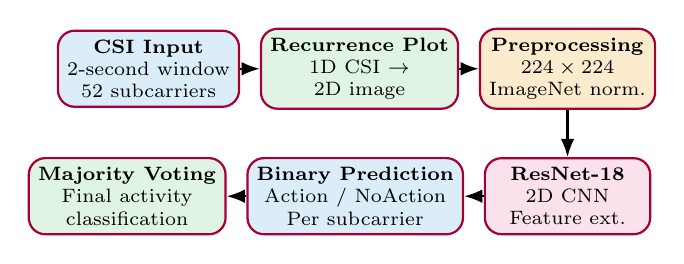
\begin{tikzpicture}[
    box/.style={
        rounded corners=6pt,
        minimum width=2.1cm,
        minimum height=0.9cm,
        align=center,
        draw=AmritaMaroon,
        thick,
        font=\scriptsize
    },
    arr/.style={-{Latex},thick}
]

% Top Row: Left to Right
\node[box,fill=LightBlue] (input)
{\textbf{CSI Input}\\
2-second window\\
52 subcarriers};

\node[box,fill=LightGreen,right=0.25cm of input] (rp)
{\textbf{Recurrence Plot}\\
1D CSI $\rightarrow$\\
2D image};

\node[box,fill=LightOrange,right=0.25cm of rp] (prep)
{\textbf{Preprocessing}\\
$224\times224$\\
ImageNet norm.};

% Bottom Row: Right to Left (Forms a clean U-Shape flow)
\node[box,fill=LightPink,below=0.6cm of prep] (resnet)
{\textbf{ResNet-18}\\
2D CNN\\
Feature ext.};

\node[box,fill=LightBlue,left=0.25cm of resnet] (prediction)
{\textbf{Binary Prediction}\\
Action / NoAction\\
Per subcarrier};

\node[box,fill=LightGreen,left=0.25cm of prediction] (voting)
{\textbf{Majority Voting}\\
Final activity\\
classification};

% Arrows mapping the U-Shape pipeline
\draw[arr] (input) -- (rp);
\draw[arr] (rp) -- (prep);
\draw[arr] (prep) -- (resnet);
\draw[arr] (resnet) -- (prediction);
\draw[arr] (prediction) -- (voting);

\end{tikzpicture}

\vspace{0.4cm}

\textbf{\color{AmritaMaroon}Training:}\\
Adam optimizer + dynamic learning-rate scheduling

\end{center}

\column{0.35\textwidth}

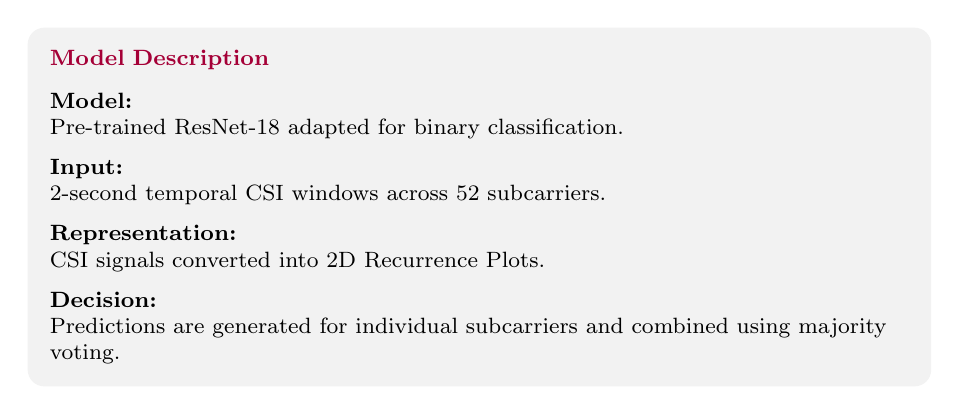
\begin{tikzpicture}
\node[
    rounded corners=6pt,
    fill=LightGray,
    inner sep=8pt,
    text width=0.9\linewidth,
    align=left,
    font=\footnotesize
] {
\textbf{\color{AmritaMaroon}Model Description}\\[6pt]

\textbf{Model:}\\
Pre-trained ResNet-18 adapted for binary classification.\\[5pt]

\textbf{Input:}\\
2-second temporal CSI windows across 52 subcarriers.\\[5pt]

\textbf{Representation:}\\
CSI signals converted into 2D Recurrence Plots.\\[5pt]

\textbf{Decision:}\\
Predictions are generated for individual subcarriers and combined using majority voting.
};
\end{tikzpicture}

\end{columns}

\end{frame}


% =========================================================
% 20. MODEL PERFORMANCE & RESULTS
% =========================================================

\begin{frame}{29. Earlier Pilot: Action vs. No-Action Results}
\roone

\begin{columns}[T,onlytextwidth]

\column{0.48\textwidth}
\begin{center}

{\small\textbf{\color{AmritaMaroon}Confusion Matrix}}

\vspace{0.08cm}

\includegraphics[
    width=0.9\linewidth,
    height=2.6cm,
    keepaspectratio
]{plot.png}

\vspace{0.15cm}

{\small\textbf{\color{AmritaMaroon}Classification Report}}

\vspace{0.08cm}

\scriptsize
\renewcommand{\arraystretch}{1.05}
\begin{tabular}{lccc}
\toprule
\textbf{Class} & \textbf{Precision} & \textbf{Recall} & \textbf{F1} \\
\midrule
NoAction & 0.93 & 0.99 & 0.96 \\
Action   & 0.99 & 0.93 & 0.96 \\
\midrule
\textbf{Overall} & \textbf{0.96} & \textbf{0.96} & \textbf{0.96} \\
\bottomrule
\end{tabular}

\end{center}

\column{0.48\textwidth}
\begin{center}

{\small\textbf{\color{AmritaMaroon}Training \& Validation Accuracy}}

\vspace{0.08cm}

\includegraphics[
    width=0.9\linewidth,
    height=2.6cm,
    keepaspectratio
]{WhatsApp Image 2026-08-13 at 11.02.06 PM.jpeg}

\vspace{0.15cm}

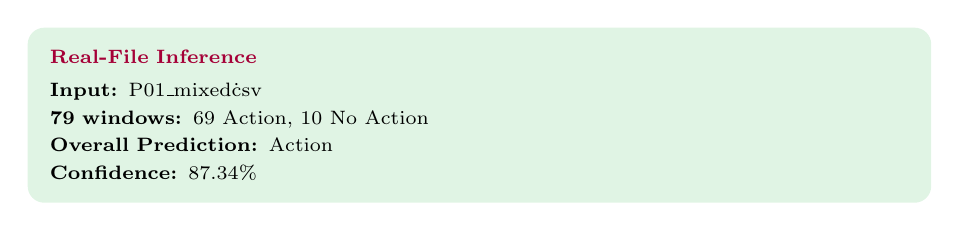
\begin{tikzpicture}
\node[
    rounded corners=6pt,
    fill=LightGreen,
    inner sep=8pt,
    text width=0.9\linewidth,
    align=left,
    font=\scriptsize
] {
\textbf{\color{AmritaMaroon}Real-File Inference}\\[4pt]
\textbf{Input:} P01\_mixed\.csv\\[2pt]
\textbf{79 windows:} 69 Action, 10 No Action\\[2pt]
\textbf{Overall Prediction:} Action\\[2pt]
\textbf{Confidence:} 87.34\%
};
\end{tikzpicture}

\end{center}
\end{columns}

\vspace{0.1cm}

\begin{center}
\textbf{\color{AmritaMaroon}Overall Classification Accuracy: 96\%}
\end{center}

\end{frame}
% =========================================================
% 22. MODEL 2: ARCHITECTURE & METHODOLOGY
% =========================================================

\begin{frame}{30. Earlier Pilot: Activity vs. Gesture Model}
\roone

\vspace{0.2cm}

\begin{columns}[T,onlytextwidth]

\column{0.62\textwidth}

\begin{center}

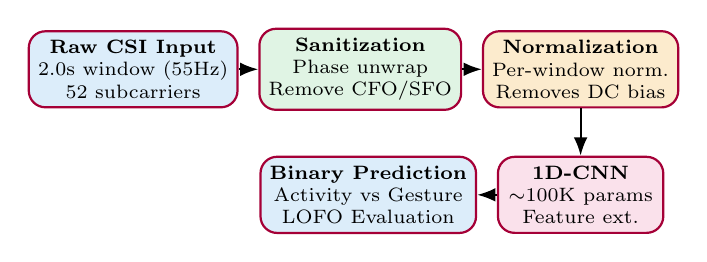
\begin{tikzpicture}[
    box/.style={
        rounded corners=6pt,
        minimum width=2.1cm,
        minimum height=0.9cm,
        align=center,
        draw=AmritaMaroon,
        thick,
        font=\scriptsize
    },
    arr/.style={-{Latex},thick}
]

% Top Row: Left to Right
\node[box,fill=LightBlue] (input)
{\textbf{Raw CSI Input}\\
2.0s window (55Hz)\\
52 subcarriers};

\node[box,fill=LightGreen,right=0.25cm of input] (sanit)
{\textbf{Sanitization}\\
Phase unwrap\\
Remove CFO/SFO};

\node[box,fill=LightOrange,right=0.25cm of sanit] (norm)
{\textbf{Normalization}\\
Per-window norm.\\
Removes DC bias};

% Bottom Row: Right to Left (Forms a clean U-Shape flow)
\node[box,fill=LightPink,below=0.6cm of norm] (cnn)
{\textbf{1D-CNN}\\
$\sim$100K params\\
Feature ext.};

\node[box,fill=LightBlue,left=0.25cm of cnn] (prediction)
{\textbf{Binary Prediction}\\
Activity vs Gesture\\
LOFO Evaluation};

% Arrows mapping the U-Shape pipeline
\draw[arr] (input) -- (sanit);
\draw[arr] (sanit) -- (norm);
\draw[arr] (norm) -- (cnn);
\draw[arr] (cnn) -- (prediction);

\end{tikzpicture}

\vspace{0.4cm}

\textbf{\color{AmritaMaroon}Training:}\\
30 Epochs + Leave-One-File-Out (LOFO) validation

\end{center}

\column{0.35\textwidth}

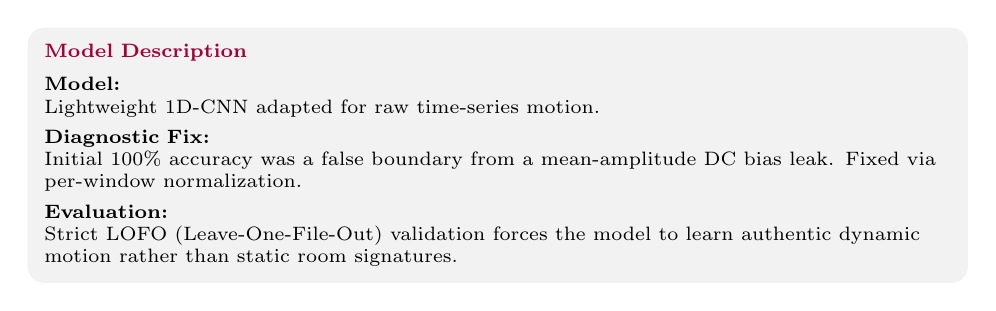
\begin{tikzpicture}
\node[
    rounded corners=6pt,
    fill=LightGray,
    inner sep=6pt,
    text width=0.95\linewidth,
    align=left,
    font=\scriptsize
] {
\textbf{\color{AmritaMaroon}Model Description}\\[4pt]

\textbf{Model:}\\
Lightweight 1D-CNN adapted for raw time-series motion.\\[3pt]

\textbf{Diagnostic Fix:}\\
Initial 100\% accuracy was a false boundary from a mean-amplitude DC bias leak. Fixed via per-window normalization.\\[3pt]

\textbf{Evaluation:}\\
Strict LOFO (Leave-One-File-Out) validation forces the model to learn authentic dynamic motion rather than static room signatures.
};
\end{tikzpicture}

\end{columns}

\end{frame}
% =========================================================
% 23. MODEL 2: PERFORMANCE & RESULTS
% =========================================================

% =========================================================
% 23. MODEL 2: PERFORMANCE & RESULTS
% =========================================================

\begin{frame}{31. Earlier Pilot: Activity vs. Gesture Results}
\roone

\vspace{-0.1cm} % Pulled up slightly to maximize space

\begin{columns}[T,onlytextwidth]

\column{0.48\textwidth}
\begin{center}

{\scriptsize\textbf{\color{AmritaMaroon}Confusion Matrix}}

\vspace{0.03cm}

\includegraphics[
    width=\linewidth,
    height=3.2cm, % Reduced height to allow the table below to fit perfectly
    keepaspectratio
]{WhatsApp Image 2026-09-06 at 6.01.55 PM.jpeg}

\vspace{0.05cm} % Tightened space between image and table

{\scriptsize\textbf{\color{AmritaMaroon}Classification Report}}

\vspace{0.02cm}

\tiny 
\renewcommand{\arraystretch}{0.95} 
\begin{tabular}{lccc}
\toprule
\textbf{Class} & \textbf{Precision} & \textbf{Recall} & \textbf{F1} \\
\midrule
Activity & 1.00 & 0.58 & 0.73 \\
Gesture  & 0.53 & 1.00 & 0.69 \\
\midrule
\textbf{Macro Avg} & \textbf{0.76} & \textbf{0.79} & \textbf{0.71} \\
\bottomrule
\end{tabular}

\end{center}

\column{0.48\textwidth}
\begin{center}

{\scriptsize\textbf{\color{AmritaMaroon}Per-Class \& Overall Metrics}}

\vspace{0.03cm}

\includegraphics[
    width=\linewidth,
    height=5.5cm, % Kept this large as requested previously
    keepaspectratio
]{WhatsApp Image 2026-09-06 at 6.01.56 PM.jpeg}

\end{center}
\end{columns}

\vspace{0.05cm} % Tightened to ensure bottom text fits comfortably

\begin{center}
\end{center}

\end{frame}
% =========================================================
% 14. CURRENT CAPABILITY VS. FUTURE EXTENSION
% =========================================================



% ------------------------------------------------


\begin{frame}{32. Current Model: Training and Evaluation}
\roone
\begin{center}
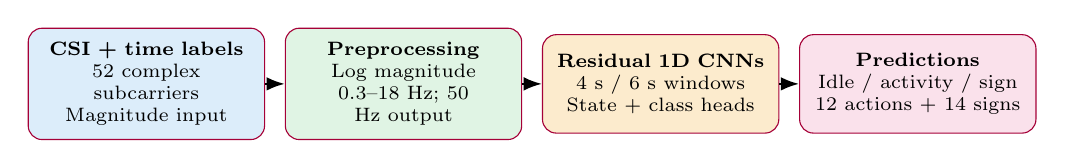
\begin{tikzpicture}[
 box/.style={draw=AmritaMaroon,rounded corners=5pt,align=center,minimum height=1.25cm,text width=2.65cm,font=\scriptsize,inner sep=5pt},
 arr/.style={-{Latex},thick}]
\node[box,fill=LightBlue] (raw) {\textbf{CSI + time labels}\\52 complex subcarriers\\Magnitude input};
\node[box,fill=LightGreen,right=0.25cm of raw] (prep) {\textbf{Preprocessing}\\Log magnitude\\0.3--18 Hz; 50 Hz output};
\node[box,fill=LightOrange,right=0.25cm of prep] (cnn) {\textbf{Residual 1D CNNs}\\4 s / 6 s windows\\State + class heads};
\node[box,fill=LightPink,right=0.25cm of cnn] (out) {\textbf{Predictions}\\Idle / activity / sign\\12 actions + 14 signs};
\draw[arr](raw)--(prep);\draw[arr](prep)--(cnn);\draw[arr](cnn)--(out);
\end{tikzpicture}
\end{center}
\vspace{0.12cm}
\begin{columns}[T,onlytextwidth]
\column{0.54\textwidth}
\footnotesize
\textbf{\color{AmritaMaroon}Five held-out-person tests}
\begin{itemize}\setlength{\itemsep}{3pt}
\item Initial fit: 3 people; validation: 1 other person.
\item Choose detector/action/sign roles on validation.
\item Refit selected networks on 4 people, two seeds.
\item Test only on the fifth person; repeat for all five.
\end{itemize}
\column{0.43\textwidth}
\footnotesize
\textbf{\color{AmritaMaroon}All-five deployment model}\\[5pt]
Two normalized four-second CNNs, one per seed, trained on all five people.\\[5pt]
Scales, masks and class order saved.\\[5pt]
Kaggle T4 $\times$2: \textbf{41.4 minutes}.
\end{columns}
\vspace{0.13cm}
\implnote{Scores come from held-out folds; the all-five refit has no independent score.
Inference is offline. ExtraTrees applies only to isolated action fusion (final weight: zero).}
\end{frame}


\begin{frame}{33. Current Results: Action Recognition}
\roone
{\footnotesize\textbf{\color{AmritaMaroon}311/628 correct (49.5\% accuracy)}
\hfill Mean held-out macro F1: \textbf{50.2\%}}
\begin{center}
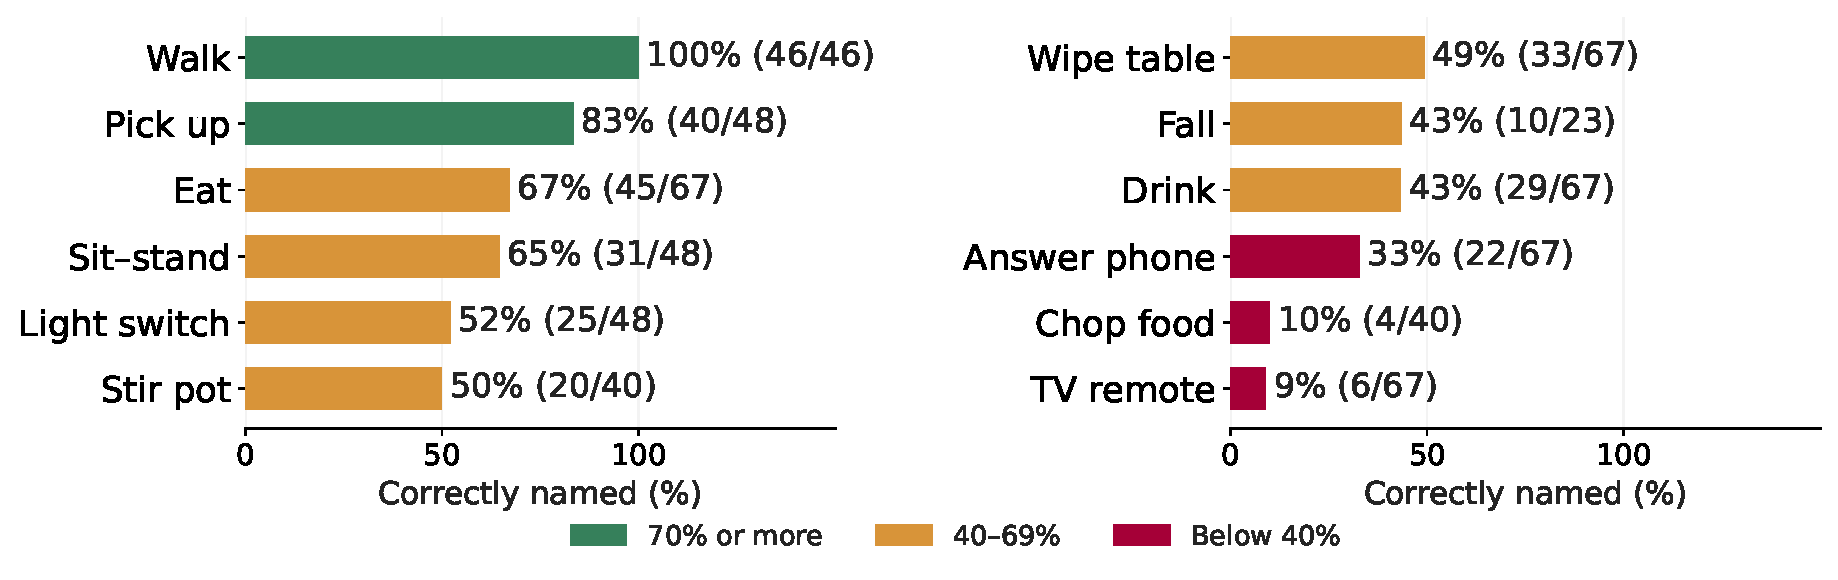
\includegraphics[width=\linewidth,height=4.45cm,keepaspectratio]{current_impl/action_class_performance.pdf}
\end{center}
\vspace{-0.08cm}
\implnote{P1--P5 isolated trials, known boundaries/type; bars show per-class recall.
\textbf{Strongest:} walk/pick up. \textbf{Weakest:} TV remote/chop/phone.
Chop/stir cover P4/P5 only.}
\end{frame}


\begin{frame}{34. Current Results: Sign Recognition}
\roone
{\footnotesize\textbf{\color{AmritaMaroon}171/490 correct (34.9\% accuracy)}
\hfill Mean held-out macro F1: \textbf{33.2\%}}
\begin{center}
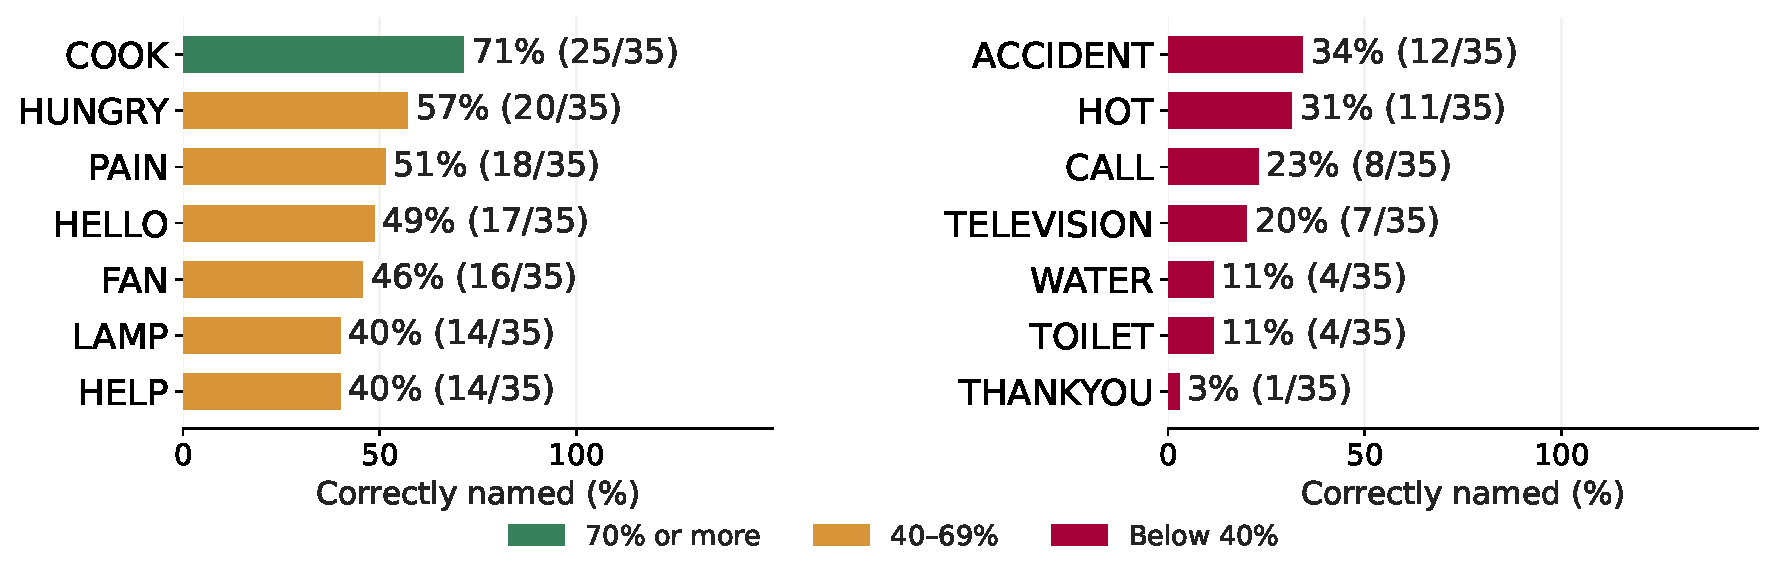
\includegraphics[width=\linewidth,height=4.45cm,keepaspectratio]{current_impl/sign_class_performance.pdf}
\end{center}
\vspace{-0.08cm}
\implnote{P1--P5: 350 standing + 140 seated trials; 35 per sign; known boundaries/type.
\textbf{Stronger:} COOK/HUNGRY/PAIN. \textbf{Weakest:} THANKYOU/WATER/TOILET.
Isolated seated signs cover P4/P5 only.}
\end{frame}


\begin{frame}{35. Current Results: Detection Threshold}
\roonefour
\begin{columns}[T,onlytextwidth]
\column{0.54\textwidth}
\footnotesize
\renewcommand{\arraystretch}{1.25}
\begin{tabular}{@{}lrr@{}}
\toprule
\textbf{Setting} & \textbf{Signs caught} & \textbf{False / hour}\\
\midrule
$\tau=0.3$: sensitive & 71.4\% & 27.5\\
$\tau=0.5$: middle & 68.9\% & 14.6\\
$\tau=0.7$: strict & 54.7\% & 10.5\\
\bottomrule
\end{tabular}
\vspace{0.25cm}

\footnotesize
Raise $\tau$ to reduce false triggers; fewer signs are caught.\\[5pt]
``Caught'' means detected, not correctly named.\\[5pt]
$\tau$ is a score cutoff, not calibrated certainty.
\column{0.43\textwidth}
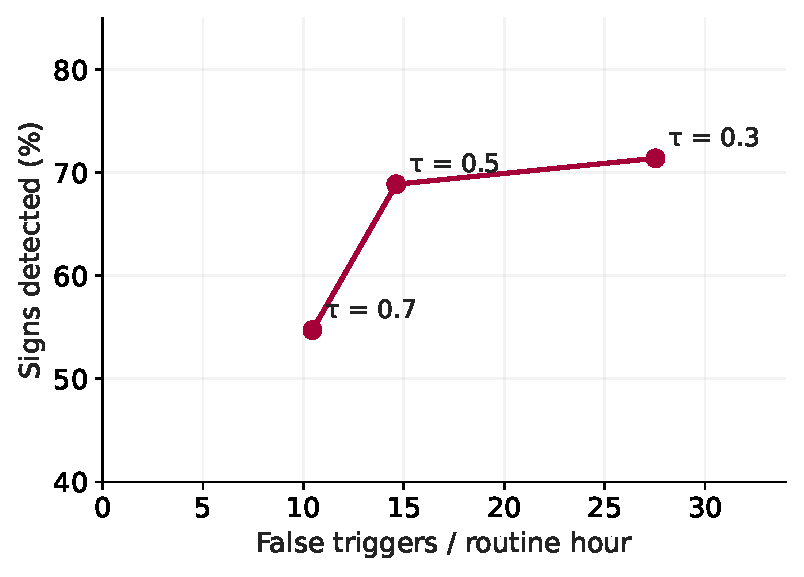
\includegraphics[width=\linewidth,height=4.25cm,keepaspectratio]{current_impl/threshold_tradeoff.pdf}
\end{columns}
\vspace{0.16cm}
\implnote{Fixed-threshold sweep: P1--P3, isolated + stories, 318 signs; mean over three people.
One-second smoothing/minimum run, one-second gap merge and $\pm$1 s matching.
Rates cover routine movement only (about 58 measured minutes), excluding idle/unknown periods.}
\end{frame}


\begin{frame}{36. Current Results: Continuous Story Recognition}
\roonefour
\begin{columns}[T,onlytextwidth]
\column{0.72\textwidth}
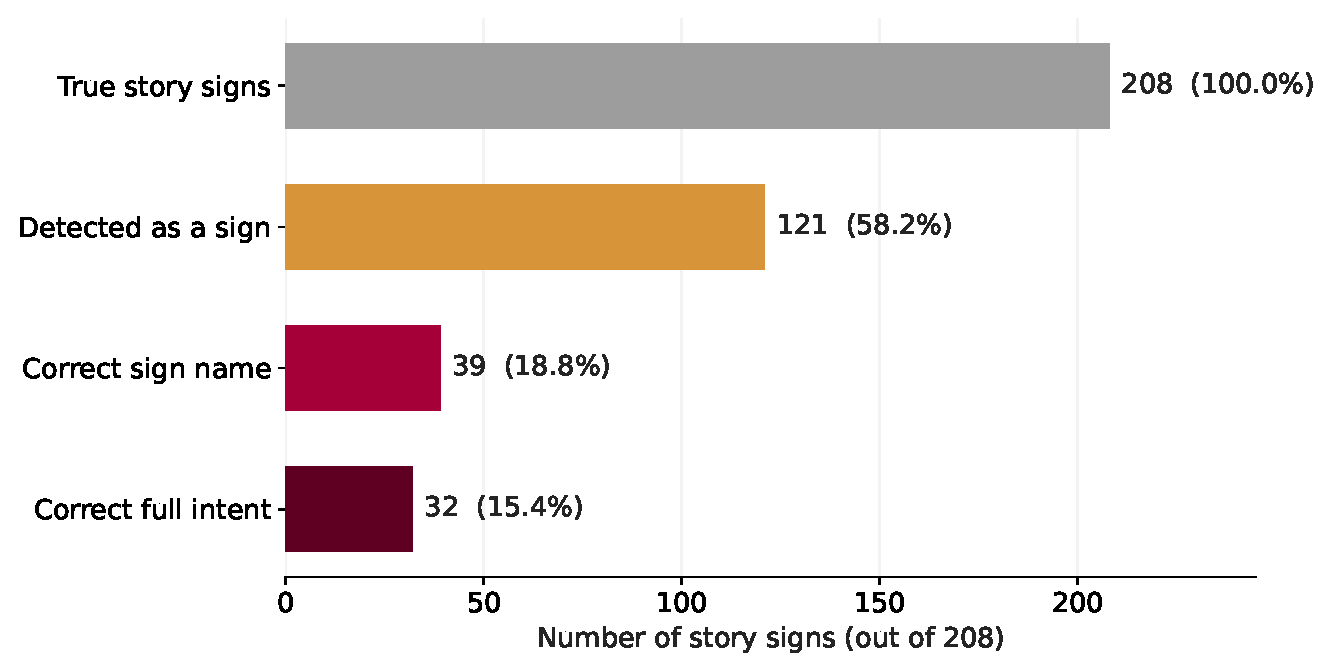
\includegraphics[width=\linewidth,height=4.55cm,keepaspectratio]{current_impl/story_recognition.pdf}
\column{0.25\textwidth}
\footnotesize
\textbf{\color{AmritaMaroon}Automatic story inference}\\[5pt]
No true sign boundaries or type are supplied.\\[6pt]
\textbf{58.2\%} of signs detected.\\[5pt]
\textbf{18.8\%} correctly named.\\[5pt]
\textbf{15.4\%} correct full intent.\\[7pt]
Continuous identity is the main remaining limitation.
\end{columns}
\vspace{0.13cm}
\implnote{All five people; validation-selected thresholds per fold; one-to-one IoU $\geq0.10$ matching.
This differs from the fixed-threshold sweep. There were 50 false triggers during 20.3 minutes of measured story routine activity.}
\end{frame}

\begin{frame}{37. MOOC / Course Selection}

\centering
\small

\renewcommand{\arraystretch}{1.35}
\setlength{\tabcolsep}{7pt}

\begin{tabular}{|c|l|p{7.5cm}|c|}
\hline
\rowcolor{red!70!black}
\color{white}\textbf{S.No} &
\color{white}\textbf{Student Name} &
\color{white}\textbf{Chosen MOOC / Course Title} &
\color{white}\textbf{Platform} \\
\hline

1 & Gowreesh B &
Certified Wireless Network Administrator (CWNA) &
Udemy \\ \hline

\rowcolor{gray!10}
2 & Adhikkesh S.K &
Basics of Digital Signal Processing for Power Engineers &
Udemy \\ \hline

3 & Amrith B &
Digital Signal Processing 2: Filtering &
Coursera \\ \hline

\rowcolor{gray!10}
4 & Adithya Ajay &
Advanced Wireless Communication Systems \\ \hline

5 & Rishiikesh S.K &
Signal Processing: Problems Solved in MATLAB and Python &
Udemy \\ \hline

\end{tabular}


\end{frame}



% =========================================================
% 22. LIMITATIONS
% =========================================================

\begin{frame}{38. Limitations}

\vspace{0.12cm}

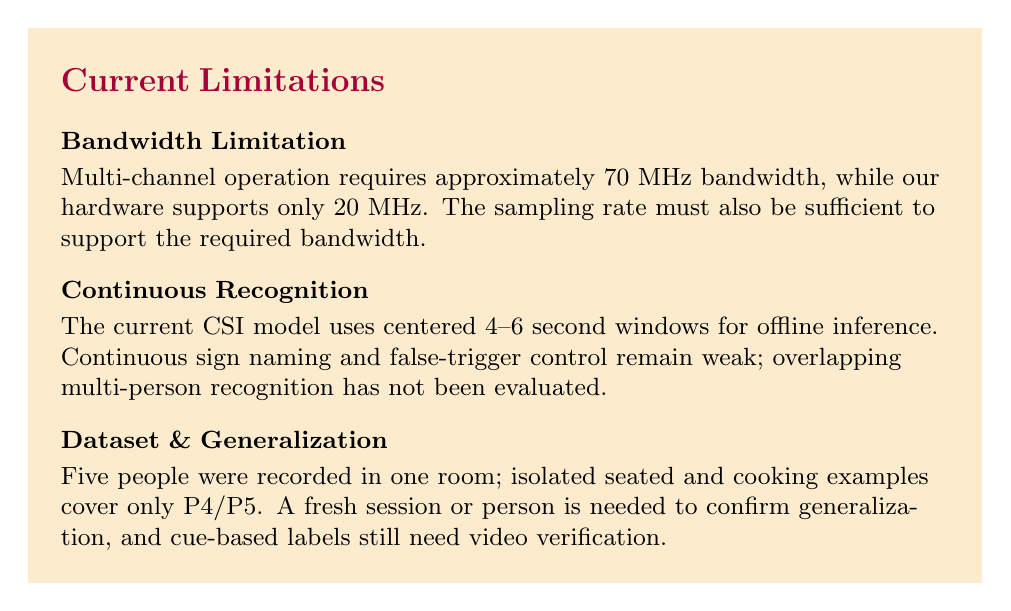
\begin{tikzpicture}
\node[
    fill=LightOrange,
    inner sep=12pt,
    text width=\linewidth-24pt,
    minimum height=5.2cm,
    align=left,
    font=\small,
    anchor=north west
] at (0,0) {

    \textbf{\large\color{AmritaMaroon}Current Limitations}\\[10pt]

    \textbf{Bandwidth Limitation}\\[2pt]
    Multi-channel operation requires approximately 70 MHz bandwidth, while our hardware supports only 20 MHz. The sampling rate must also be sufficient to support the required bandwidth.\\[8pt]

    \textbf{Continuous Recognition}\\[2pt]
    The current CSI model uses centered 4--6 second windows for offline inference. Continuous sign naming and false-trigger control remain weak; overlapping multi-person recognition has not been evaluated.\\[8pt]

    \textbf{Dataset \& Generalization}\\[2pt]
    Five people were recorded in one room; isolated seated and cooking examples cover only P4/P5. A fresh session or person is needed to confirm generalization, and cue-based labels still need video verification.
};

\end{tikzpicture}

\end{frame}
% =========================================================
% 23. REFERENCES
% CLEAN IEEE STYLE -- 3 SLIDES
% =========================================================

% =========================================================
% REFERENCES (1/3)
% =========================================================

\begin{frame}{39. References (1/3)}

\footnotesize
\color{black}
\raggedright

\begin{list}
    {}
    {
        \setlength{\leftmargin}{0.45cm}
        \setlength{\labelwidth}{0cm}
        \setlength{\labelsep}{0.10cm}
        \setlength{\itemsep}{8pt}
        \setlength{\parsep}{0pt}
        \setlength{\topsep}{0pt}
    }

\item[\textbf{[1]}]
X. Chen \emph{et al.}, ``Towards LLM-Powered Ambient Sensor Based
Multi-Person Human Activity Recognition (LAHAR),'' 2024.
\hspace{2pt}
\href{https://ieeexplore.ieee.org/document/10763542/}
{\textcolor{AmritaMaroon}{[Link]}}

\item[\textbf{[2]}]
Li \emph{et al.}, ``Multiperson Activity Recognition and Tracking
Based on Skeletal Keypoint Detection,'' 2024.
\hspace{2pt}
\href{https://www.researchgate.net/publication/374189243_Multiperson_Activity_Recognition_and_Tracking_Based_on_Skeletal_Keypoint_Detection}
{\textcolor{AmritaMaroon}{[Link]}}

\item[\textbf{[3]}]
Hiremath \emph{et al.}, ``Maintenance Required: Updating and Extending
Bootstrapped Human Activity Recognition Systems for Smart Homes,'' 2024.
\hspace{2pt}
\href{https://arxiv.org/pdf/2406.14446}
{\textcolor{AmritaMaroon}{[Link]}}

\item[\textbf{[4]}]
H. Wen \emph{et al.}, ``Improving Skeleton-based Action Recognition
with Interactive Object Information,'' 2025.
\hspace{2pt}
\href{https://arxiv.org/abs/2501.05066}
{\textcolor{AmritaMaroon}{[Link]}}

\end{list}

\end{frame}


% =========================================================
% REFERENCES (2/3)
% =========================================================

\begin{frame}{40. References (2/3)}

\footnotesize
\color{black}
\raggedright

\begin{list}
    {}
    {
        \setlength{\leftmargin}{0.45cm}
        \setlength{\labelwidth}{0cm}
        \setlength{\labelsep}{0.10cm}
        \setlength{\itemsep}{8pt}
        \setlength{\parsep}{0pt}
        \setlength{\topsep}{0pt}
    }

\item[\textbf{[5]}]
``Attention-based Contrastive Learning for HAR (AttCLHAR),''
2024.
\hspace{2pt}
\href{https://pmc.ncbi.nlm.nih.gov/articles/PMC10857438/}
{\textcolor{AmritaMaroon}{[Link]}}

\item[\textbf{[6]}]
``Occlusion-Aware Hypergraph Reasoning for Skeleton Action Recognition
(OAHR),'' 2024.
\hspace{2pt}
\href{https://www.researchgate.net/publication/363910427_Revisiting_Skeleton-based_Action_Recognition}
{\textcolor{AmritaMaroon}{[Link]}}

\item[\textbf{[7]}]
Y. Ma \emph{et al.}, ``SignFi: Sign Language Recognition Using WiFi,''
\emph{Proc. ACM Interact. Mob. Wearable Ubiquitous Technol.},
vol. 2, no. 1, pp. 1--21, 2018.
\hspace{2pt}
\href{https://dl.acm.org/doi/10.1145/3191755}
{\textcolor{AmritaMaroon}{[Link]}}

\item[\textbf{[8]}]
L. Hu \emph{et al.}, ``Continuous Sign Language Recognition With
Correlation Network,'' in \emph{Proc. IEEE/CVF Conf. Comput. Vis.
Pattern Recognit. (CVPR)}, 2023, pp. 2529--2539.
\hspace{2pt}
\href{https://openaccess.thecvf.com/content/CVPR2023/html/Hu_Continuous_Sign_Language_Recognition_With_Correlation_Network_CVPR_2023_paper.html}
{\textcolor{AmritaMaroon}{[Link]}}

\end{list}

\end{frame}


% =========================================================
% REFERENCES (3/3)
% =========================================================

\begin{frame}{41. References (3/3)}

\footnotesize
\color{black}
\raggedright

\begin{list}
    {}
    {
        \setlength{\leftmargin}{0.45cm}
        \setlength{\labelwidth}{0cm}
        \setlength{\labelsep}{0.10cm}
        \setlength{\itemsep}{8pt}
        \setlength{\parsep}{0pt}
        \setlength{\topsep}{0pt}
    }

\item[\textbf{[9]}]
J. Gong \emph{et al.}, ``LLMs are Good Sign Language Translators,''
in \emph{Proc. IEEE/CVF Conf. Comput. Vis. Pattern Recognit. (CVPR)},
2024, pp. 18362--18372.
\hspace{2pt}
\href{https://openaccess.thecvf.com/content/CVPR2024/html/Gong_LLMs_are_Good_Sign_Language_Translators_CVPR_2024_paper.html}
{\textcolor{AmritaMaroon}{[Link]}}

\item[\textbf{[10]}]
H. Wang \emph{et al.}, ``Wi-SL: Translating Continuous Sign Language
into Text Using Ambient WiFi Signals,'' 2023.
\hspace{2pt}
\href{https://www.mdpi.com/1424-8220/20/14/4025}
{\textcolor{AmritaMaroon}{[Link]}}

\item[\textbf{[11]}]
Liu \emph{et al.}, ``WatchSign: Daily Sign Language Tracking Utilizing
Commercial Smartwatch IMU Sensors,'' 2023.

\item[\textbf{[12]}]
Y. Gu \emph{et al.}, ``End-to-End Continuous Sentence-Level ASL
Translation Capturing Whole-Arm Inertial Data,'' 2024.
\hspace{2pt}
\href{https://www.mdpi.com/1424-8220/24/2/453}
{\textcolor{AmritaMaroon}{[Link]}}

\end{list}

\end{frame}

\end{document}